\documentclass[a4paper,11pt]{article}
\pdfoutput=1 % if your are submitting a pdflatex (i.e. if you have
         % images in pdf, png or jpg format)

\usepackage{jcappub} % for details on the use of the package, please
                 % see the JCAP-author-manual

\usepackage{hyperref}
\usepackage{amsmath}

\usepackage[english,activeacute]{babel} 
\usepackage[toc,page]{appendix}
\usepackage{graphicx}
\usepackage{color}
\usepackage{tensor}

\usepackage{xcolor}
\usepackage{graphicx}
\usepackage{colortbl}
\usepackage{placeins}
\usepackage[margin=2.5cm]{geometry}
\usepackage{multirow}

\usepackage[utf8]{inputenc}

% command for co-polarized
\newcommand{\co}{\mathbin{\|}}

% command for cross-polarized
\newcommand{\cx}{\mathbin{\times}}


\title{\boldmath Pixel space convolution for cosmic microwave background experiments}


%% %simple case: 2 authors, same institution
%% \author{A. Uthor}
%% \author{and A. Nother Author}
%% \affiliation{Institution,\\Address, Country}

% more complex case: 4 authors, 3 institutions, 2 footnotes
\author[a]{P. Flux\'a, }
\author[b]{M.K. Brewer, }
\author[a]{R. D\"unner.}

% The "\note" macro will give a warning: "Ignoring empty anchor..."
% you can safely ignore it.

\affiliation[a]{Instituto de Astrof\'isica, Pontificia Universidad Cat\'olica de Chile ,\\Vicu\~na Mackenna 4860, Chile}
\affiliation[b]{Department of Astronomy, Johns Hopkins University,\\Baltimore MD, USA}

% e-mail addresses: one for each author, in the same order as the authors
\emailAdd{pedro@fluxanet.net}
\emailAdd{brewer@astro.umass.edu}
\emailAdd{rdunner@astro.puc.cl}

\abstract{
	Cosmic microwave background experiments have experienced an exponential increase in complexity, data size and sensitivity. Current and future experiments aim at characterizing the B-mode power spectrum which, due to its faintness, will require extreme control over systematic effects. One such effect might arise from the complex coupling between the telescope beam and its scanning strategy. In this work, we present a new software tool, the Pixel Space COnvolver, PISCO, capable of producing mock data streams for a general CMB experiment. We show results of an application of PISCO to the Cosmology Large Angular Scale Surveryor, and its Q-band telescope.  }

\begin{document}
\maketitle
\flushbottom

% enable numbering of equations that considers the section number
%\numberwithin{equation}{section}

\section{Introduction}

% gives the width of the current document in pts
\showthe\textwidth

The study of the cosmic microwave background (CMB) in the last few decades has lead to major advances in Cosmology. In particular, the study of the temperature and polarization anisotropy field has allowed us to achieve percent level constraints on cosmological parameters, favoring a universe dominated by cold dark matter plus a cosmological constant ($\Lambda$CDM), known today as the standard model of Cosmology {\color{red} (cite most relevant papers including WMAP and Planck)}. Current efforts are mostly focused on the polarization anisotropy field, as it promises to provide independent constraints on the very early stages of the Universe. At these very first moments, the leading theory claims that the Universe exponentially expanded nearly 60 e-folds in a process called inflation, becoming the flat, homogeneous and isotropic Universe that we see today. If true, gravitational waves generated by this expansion would have later interacted with the surface of last scatter, leaving a unique imprint in the polarization field which should be observable today.

CMB anisotropies form a Gaussian field on the sky, being nearly 10\% polarized. The latter can be modeled as a spin-2 field, which is separable in two orthogonal components: a curl-free component called E-mode, and a divergence-free component called B-mode. In the absence of gravitational waves, the polarization field would contain only E-modes, which would be partially turned into B-modes by gravitational waves acting during the epochs of recombination and reionization. The resulting B-mode field would be one or two orders of magnitude lower than the E-mode signal, being very faint and difficult to measure. Moreover, recent results show that this signal lies below other foreground signals like gravitational lensing distortions induced by the matter distribution and polarized emissions from the interstellar medium {\color{red}(add cites)}. Thus, detecting the primordial B-mode signal has become a major technical challenge.

Another source of confusion is experimental systematic effects. The tremendous increase in sensitivity of CMB experiments has brought into play a long list of instrumental and observational effects, which need to be properly incorporated into the data reduction process, as well as for the design of future experiments. Being an extended signal on the sky, understanding the effects of the detailed polarized antenna response of the telescope, and how it gets convolved with the sky signal (scan strategy), is key, as it can directly affect the scientific results.

The main beam is where most of the radiation is captured by the antenna, and thus the effects of the beam shape and polarization have been extensively studied. 
%Analytic techniques
It has been shown that the effect of symmetrical beams with smooth profiles can be analytically accounted for when computing the power spectra of CMB maps (see \cite{2003ApJS..148...39P}).
However, beam and pointing mismatch can produce leakage between temperature and polarization (T to P), or between E-modes and B-modes (P to P). The impact of these effects on the maps, power spectra and scientific results, together with mitigation techniques, have been proposed by \cite{PhysRevD.77.083003, 2007MNRAS.376.1767O, 2015JCAP...03..048D}.

The problem becomes much more complicated when sidelobes are included, forcing the use of numerical methods to understand their effects.
Several of these techniques rely on harmonic space representations of the beam, the sky and the scan strategy (\cite{2001PhRvD..63l3002W,2000PhRvD..62l3002C}). Harmonic space algorithms can also exploit redundancies in the computation that allow Fast Fourier Transform (FFT) techniques to be used. An excellent description of FFT-based algorithms, as well an implementation and application to a realistic CMB experiment is given in \cite{2018arXiv180905034D}. On the other hand, pixel space algorithms can account for time-varying effects, like transient events on the sky model, modulation techniques and optical distortions. The work of \cite{2011ApJS..193....5M} describes such an implementation, and its application to the Planck satellite mission.

%Planks approach ... 
The Planck experiment developed Full Focal Plane (FFP) simulations (see \cite{2016A&A...594A..12P}). At the time they were performed, FFP simulations took more than four million CPU-hours on a world-class supercomputer, and required almost 18 TB of storage. FFP simulations included very detailed noise models of the Planck mission and helped, among other things, to provide excellent constraints on the the cosmological parameters and their associated statistical errors (see \cite{2016A&A...594A..13P}). FFP simulations showed that effort on improving tools aimed at simulating CMB experiments will become valuable for current and future missions.

%O'dea approach ...



In this work, we describe the algorithm and prototype implementation of a new CMB computer simulation code, the Pixel Space COnvolver (PISCO). PISCO has the capability of accounting for arbitrary shaped, time-varying beams and sky models. Full polarization treatment of the beam properties is based on the work presented in \cite{2007MNRAS.376.1767O}. PISCO also exploits the massively parallel architecture of Graphics Processing Units (GPU), via the CUDA platform, and was designed from scratch to take advantage of HPC environments.

This paper is organized as follows. 
\S\ref{sec::coordinate-systems} contains a description of the coordinate system and geometrical transformations used to model an antenna pointing at the sky.
\S\ref{sec::antennas} presents a brief introduction to antenna theory. 
\S\ref{sec::pixel_conv} describes the algorithm used by PISCO, as well as a prototype implementation. 
\S\ref{sec::validation} presents validation tests to assess the performance of PISCO. 
\S\ref{sec::realistic_cmb_experiment} provides an example application of PISCO to CLASS (\cite{2016SPIE.9914E..1KH}). 
The paper concludes with a brief discussion of the results obtained in \S\ref{sec::conclusions}.

%
\section{Coordinates}
\label{sec::coordinate-systems}

\subsection{Definitions}

\begin{figure*}
	\centering
	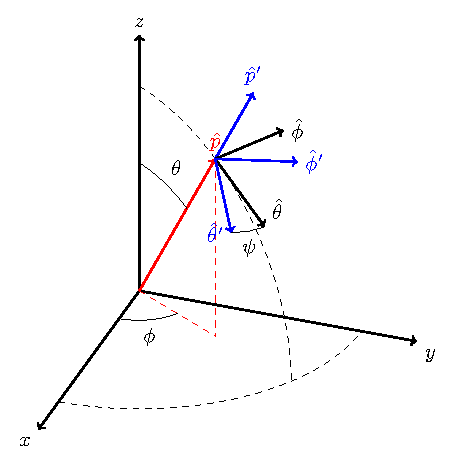
\includegraphics[width=0.47\linewidth]{tikz/sky_basis}	
	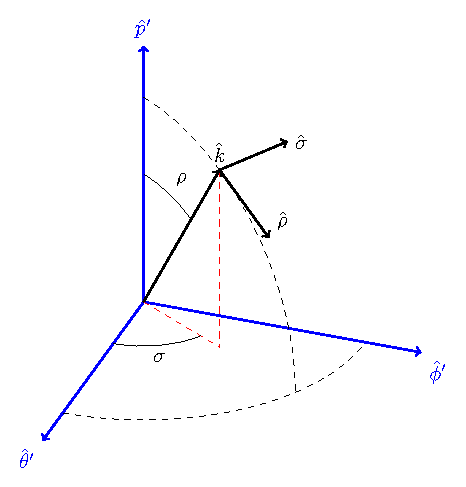
\includegraphics[width=0.47\linewidth]{tikz/beam_basis}
	\caption{Left panel: sky basis. The sky basis is a generic spherical coordinate system. $\hat{x}$, $\hat{y}$ and $\hat{z}$ form an orthonormal basis. Unit vector $\hat{p}$ is defined by its spherical coordinates, co-latitude $\theta$ and longitude $\phi$. Co-latitude increases from the north pole towards the south pole. Longitude increases from west to east. Tangent vectors at $\hat{p}$, $\hat{\theta}$ and $\hat{\phi}$, can be rotated around $\hat{p}$ by angle $\psi$ to generate vectors $\hat{\theta}'$ and $\hat{\phi}'$. Note an observer looking towards the sky along $\hat{p}$ will measure angle $\psi$ as increasing clockwise from South. Right panel: antenna basis. The antenna basis is another orthonormal basis, very much like the sky basis. A unit vector $\hat{k}$ is described by $\rho$ (co-latitude) and $\sigma$ (longitude). Tangent vectors at $\hat{k}$ are $\hat{\rho}$ and $\hat{\sigma}$. }
	\label{fig::sky_basis} 
\end{figure*}

Since PISCO performs the convolution of the polarized antenna response with the sky in ``real'' domain, it makes extensive use of coordinate transformations. These operations can be described by the use of two complementary spherical coordinate systems, which are described in figure \ref{fig::sky_basis}. The first coordinate system corresponds to the \textsl{sky basis}. Unit base vectors of these coordinate system are $\hat{x}$, $\hat{y}$ and $\hat{z}$. For convenience, the antenna pointing in the sky basis will be described as a 3-tuple $\bar{q}$, so that an antenna aiming at co-latitude $\theta_0$ and longitude $\phi_0$, with position angle $\psi_0$ has a pointing 

\begin{equation}
\begin{aligned}
\bar{q}_0= (\theta_0,\phi_0,\psi_0)
\end{aligned}
\end{equation}

Then the \textsl{pointing direction}, denoted by vector $\hat{p}_0$, can be expressed as a linear combination of base vectors and spherical coordinates $(\theta_0,\phi_0)$ via

\begin{equation}
\begin{aligned}
\hat{p}_0 = \sin(\theta_0)\cos(\phi_0) \hat{x} + \sin(\theta_0)\sin(\phi_0) \hat{y} + \cos(\theta_0) \hat{z}
\end{aligned}
\label{eq::p_sky_basis}
\end{equation}

The vectors $\hat{\theta}_0$ and $\hat{\phi}_0$ are computed using

\begin{eqnarray}
\begin{aligned}
\hat{\theta}_0 &=&  \cos(\theta_0) \cos(\phi_0) \hat{x} + \cos(\theta_0)\sin(\phi_0) \hat{y} - \sin(\theta_0) \hat{z} \\
\hat{\phi}_0   &=&              -\sin(\phi_0) \hat{x} +             \cos(\phi_0) \hat{y}
\end{aligned}
\label{eq::tangent_sky_basis}
\end{eqnarray}

These vectors can be used to build a second coordinate system, the \textsl{antenna basis}. Given an antenna pointing $\bar{q}_0$, the antenna basis base vectors can be written in term of sky basis coordinates as 

\begin{eqnarray}
%\begin{aligned}
\hat{p}'_0      &=&  \hat{p}_0 \\
\hat{\theta}'_0 &=&  \cos(\psi_0)\hat{\theta}_0 + \sin(\psi_0)\hat{\phi}_0 \\
\hat{\phi}'_0   &=& -\sin(\psi_0)\hat{\theta}_0 + \cos(\psi_0)\hat{\phi}_0
%\end{aligned} 
\label{eq::antenna_base_vectors}
\end{eqnarray}

In the antenna basis, coordinates analog to sky basis co-latitude and longitude are $\rho$ and $\sigma$, respectively. As in equation \ref{eq::p_sky_basis}, a vector $\hat{k}$ can be similarly written in terms of antenna basis coordinates as

\begin{equation}
\begin{aligned}
\hat{k}       &=&  \sin(\rho)\cos(\sigma)\hat{\theta}'_0 + \sin(\rho)\sin(\sigma) \hat{\phi}'_0 + \cos(\rho) \hat{p}'_0 
\end{aligned}
\end{equation}

\noindent
while vectors analog to the ones described by equation \ref{eq::tangent_sky_basis} are

\begin{eqnarray}
\begin{aligned}
\hat{\rho}    &=&  \cos(\rho)\cos(\sigma)\hat{\theta}'_0 + \sin(\rho)\sin(\sigma) \hat{\phi}'_0 - \sin(\rho) \hat{p}'_0 \\
\hat{\sigma}  &=& -\sin(\sigma)\hat{\theta}'_0 + \cos(\sigma)\hat{\phi}'_0
\end{aligned}
\end{eqnarray}

In many situations, antennas are equipped with polarization sensitive devices. The direction on the sky for which the device has maximum sensitivity to linearly polarized radiation is called co-polarization, denoted by $\hat{e}_{\co}$. The perpendicular direction, known as cross-polarization, is denoted by $\hat{e}_{\cx}$.
Because polarization is defined in the sky basis (see Figure \ref{fig::cmbcoordconvention}), a polarization sensitive antenna must compensate for the apparent rotation of its own polarization basis with respect to the sky. This can be accomplished by rotating the incoming Stokes vector by the angle between $\hat{e}_{\co}$ and $\hat{\theta}$, namely

\begin{equation}
\psi(\rho,\sigma) = \arctan \left( \frac{ |\hat{e}_{\co} \times \hat{\theta}| }{ \hat{e}_{\co} \cdot \hat{\theta} } \right)
\label{eq::psi}
\end{equation}

See Appendix A for details on the definition of co-polarization and cross-polarization that PISCO uses and the computation of $\psi(\rho,\sigma)$ using spherical trigonometry.

\begin{figure}
	\centering
	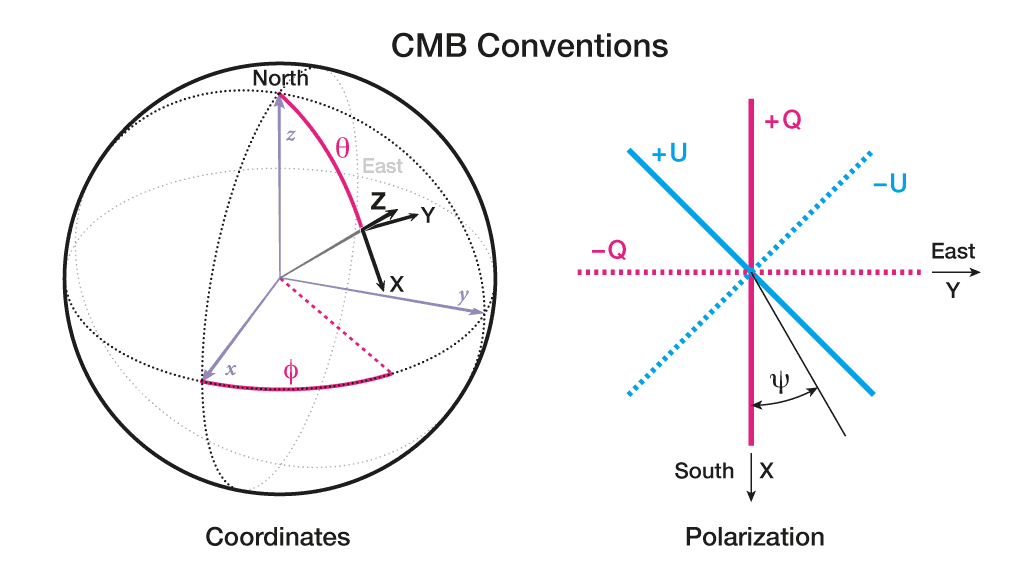
\includegraphics[width=0.7\linewidth]{figures/cmb_coord_convention}
	\caption{Figure showing the convention used for polarization among the CMB community. In this figure, $z$ is parallel to $\hat{p}_0$, $x$ is parallel to $\hat{\theta}$ and $y$ points along $\hat{\phi}$. $\psi$ is the angle between the antenna ``up'' direction, and $x$ ($\hat{\theta}$). The sign conventions of Stokes parameters $Q$ and $U$ used by the CMB community are: positive $Q$ if the polarization vector is aligned with $\hat(\theta)$ (North-South direction), negative $Q$ if the polarization vector is aligned with $\hat{\phi}$ (East-West direction), positive $U$ is aligned with $(\pm(\hat{\phi} + \hat{\theta})/\sqrt{2} )$ (North/West-South/East direction), and negative $U$ is aligned with $(\pm(\hat{\phi} - \hat{\theta})/\sqrt{2} )$ (North/East-South/West direction). Note that the right-most panel of this figure corresponds to an observer looking \textsl{towards Earth}. Figure source: \href{https://lambda.gsfc.nasa.gov/product/about/pol_convention.cfm}{LAMBDA website}}
	\label{fig::cmbcoordconvention}
\end{figure}

\section{A polarized model for antennas}
\label{sec::antennas}

The properties of an antenna equipped with detectors that are insensitive to polarization can be fully characterized by its beam. The beam is defined in terms of the antenna angular power density distribution $U(\rho,\sigma)$ via

\begin{equation}
\begin{aligned}
b(\rho, \sigma) = \frac{ U(\rho, \sigma) }{ \mathrm{MAX}\left[ U(\rho,\sigma) \right] }  =  \frac{ U(\rho, \sigma) }{ U(0,0) } \, .
\end{aligned}
\label{eq::beam_def}
\end{equation}

\noindent
A standard quantification of an antenna's ability to direct power to a particular region of the sky is given by the beam solid angle $\Omega$, calculated as

\begin{equation}
\begin{aligned}
\Omega = \int_{4\pi} b(\rho,\sigma) \, \mathrm{d} \Omega \, .
\end{aligned}
\label{eq::omega_def}
\end{equation}

These concepts fully characterize a lossless antenna in the case it is not sensitive to polarization. In the more general case where the antenna is used to measure polarization, its polarizing properties can be obtained by combining the concept of a beam with the Mueller matrix formalism. Mueller matrices are widely used to quantify the effect that an optical element has on the polarization state of incoming light. This process is modeled by the multiplication of $4\times4$ matrix $\mathbf{M}$ with a Stokes vector $S_{\mathrm{in}}$ such that the polarization state of light after the interaction with a given optical element becomes

\begin{equation}
\begin{aligned}
S_{\mathrm{out}} = \mathbf{M} S_{\mathrm{in}}
\end{aligned}
\end{equation}

\noindent
As described in the work of \cite{piepmeier_long_njoku_2008} and \cite{2007MNRAS.376.1767O}, antennas can be modeled using Mueller matrices. PISCO is based on the work of \cite{2007MNRAS.376.1767O}, since it describes a formalism that is more suitable to be applied to CMB experiments. We note the original paper names ``beam Mueller fields'' to this extended definition of a antenna beam. In this work, we refer to it as a beam tensor, or \textsl{beamsor} for short, to emphasize the multi-dimensional nature of this mathematical entity. 

A beamsor can be interpreted as a field of Mueller matrices such that for each direction $(\rho,\sigma)$, there is an associated Mueller matrix that quantifies the coupling between the antenna and a Stokes vector coming from $(\rho,\sigma)$. We will denote a beamsor by letter $B = B(\rho,\sigma)$. At every antenna basis direction, $B$ is a $4\times4$ matrix in the form

\begin{equation}
\begin{aligned}
B(\rho,\sigma) = \frac{1}{\tilde{\Omega}}
\begin{bmatrix}
B_{TT} & B_{QT} & B_{UT} & B_{VT}\\
B_{TQ} & B_{QQ} & B_{UQ} & B_{VQ}\\
B_{TU} & B_{QU} & B_{UU} & B_{VU}\\
B_{TV} & B_{QV} & B_{UV} & B_{VV}
\end{bmatrix}
\end{aligned}
\label{eq::beamsor}
\end{equation}

\noindent
where $\tilde{\Omega}$ is a normalization factor

\begin{equation}
\begin{aligned}
\tilde{\Omega} = \int_{4\pi} B_{TT}(\rho,\sigma) \, \mathrm{d} \Omega
\end{aligned}
\end{equation}

\noindent
and the elements of $B$ are defined in Appendix B. 

\section{Measuring the sky with polarization sensitive antennas}

\subsection{Continuous case}

In order to model the process by which a polarization sensitive detector transforms electromagnetic radiation into current or voltage, we used the formalism described in \cite{2007MNRAS.376.1767O}. In Mueller matrix space, a partially polarized, total power detection device corresponds to the following row-vector 

\begin{equation}
\begin{aligned}
\tensor{D}{_{i}}(\zeta,\epsilon,s) = \frac{s}{2} \left[(1 + \epsilon), (1 - \epsilon)\cos(2\zeta), (1 - \epsilon)\sin(2\zeta), 0 \right]
\end{aligned}
\label{eq::M_pol}
\end{equation}

\noindent
where $1 - \epsilon$ is the polarization efficiency, $s$ is the voltage responsivity of the detector and the angle $\zeta$ is the orientation of the polarization sensitivity axis of the linear polarizer with respect to $\hat{e}_{\co}$ at beam center. The process of taking a total power measurement on a Stokes vector $\tensor{S}{^{i}}$ can then be modeled as

\begin{equation}
\begin{aligned}
d = \tensor{D}{_{i}} \tensor{S}{^{i}}
\end{aligned}
\label{eq::total_power_measurement}
\end{equation}

We note that $\tensor{S}{^{i}}$ is, in turn, the convolution between the antenna beamsor and the polarized sky. Then, the complete formula describing the measurement taken by a linearly polarized, total power detector coupled to an antenna pointing along $\hat{p}$ with position angle $\psi_0$ becomes

\begin{equation}
\begin{aligned}
d(\bar{q}_0) = \tensor{D}{_{i}}(\zeta,\epsilon,s) \int_{4\pi} \tensor{B}{^{i}_{j} } \left[ \tensor{\Lambda}{^{j}_{k} } \tensor{S}{^{k}} \right ] \, \mathbf{d} \Omega
\end{aligned}
\label{eq::pisco_equation_cont}
\end{equation}

\noindent
where $(i,j) = T,Q,U,V$, and $B$ is aligned with $(\hat{p},\psi_0)$ (see Appendix A). Rotation of the sky to antenna polarization basis is carried out by $\Lambda$, which is a matrix field in the form

\begin{equation}
\begin{aligned}
\Lambda =
\begin{bmatrix}
1  & 0 & 0 & 0\\
0  & \cos(2\psi) & \sin(2\psi) & 0\\
0  &-\sin(2\psi) & \cos(2\psi) & 0\\
0  & 0 & 0 & 1
\end{bmatrix}
\end{aligned}
\label{eq::lambda_operator}
\end{equation}

\subsection{Pixelated case}
\label{sec::pixel_conv}

In order to calculate the result of equation \ref{eq::pisco_equation_cont} using a computer, we can no longer use continuous distributions, so we need to use pixelated versions of both the beamsor and sky model. Both the sky model $S$ and beamsor $B$ must then be transformed into a matrix of $N_b$ (number of pixels in the beamsor) and $N_s$ (number of pixels in the sky model) entries, respectively. We will denote the $k$-th pixel of the ``pixelated'' beamsor $B$ (sky $S$) as $\tensor[_k]{B}{}$ ($\tensor[_k]{S}{}$). It is worth noting that the TOD generation routine run by PISCO requires both the beamsor and sky model to be already pixelated. With the above in mind, we can write equation \ref{eq::pisco_equation_cont} for the pixelated case as

\begin{equation}
\begin{aligned}
d(\bar{q}_0) = \
\tensor{D}{_{i}}(\zeta,\epsilon,s) \
\sum_{k=1}^{N_s} \
\tensor[_k]{B}{^i_j} \
\tensor[_k]{\Lambda}{^j_m} \
\tensor[_k]{S}{^m}
\end{aligned}
\label{eq::discrete_beam_conv_tensor}
\end{equation}

\noindent
where $B$ has been properly re-pixelated via interpolation to be aligned with the sky according to $\bar{q}_0$ using the equations presented in Appendix A.

\section{PISCO}

The \textbf{PI}xel \textbf{S}pace \textbf{CO}nvolver (PISCO) is a tool with the capability of generating synthetic Time Ordered Data (TOD) provided a model for the beamsor, the scanning strategy of the mission and a sky model. In this section, we present a pathfinder implementation of PISCO ($p$-PISCO) that exploits the massively parallel architecture of modern GPU systems.

\subsection{General description}

PISCO is the software tool in charge of generating mock TOD given a beamsor, a sky model and a scanning strategy. A diagram showing the general workings of PISCO is shown in Figure \ref{fig::pisco_flow}. PISCO receives as input a sky model in the form of 4 maps representing Stokes parameters $I,Q,U$ and $V$, a beamsor, pointing and focal plane information. PISCO stores the beamsor elements and sky model as HEALPix (see \cite{2005ApJ...622..759G}) maps. HEALPix was chosen because it is widely used among the CMB community, and because it naturally handles the closed surface topology of the sphere. HEALPix also provides equal area pixels, which is a desirable feature when computing convolution in pixel space. The focal plane specifications are only needed if multiple detectors are being included in the pointing stream, as PISCO needs the the angle $\zeta$ of each detector to compute equation \ref{eq::discrete_beam_conv_tensor}. All the inputs are sent to the TOD generation function, which returns the data streams. At this point, the data can either be saved to disk or sent to a map-making code. This last step is preferred as, usually, input-output operations are time consuming. Finally, maps can be analyzed using external tools to calculate the power spectra.

\begin{figure}
	\centering
	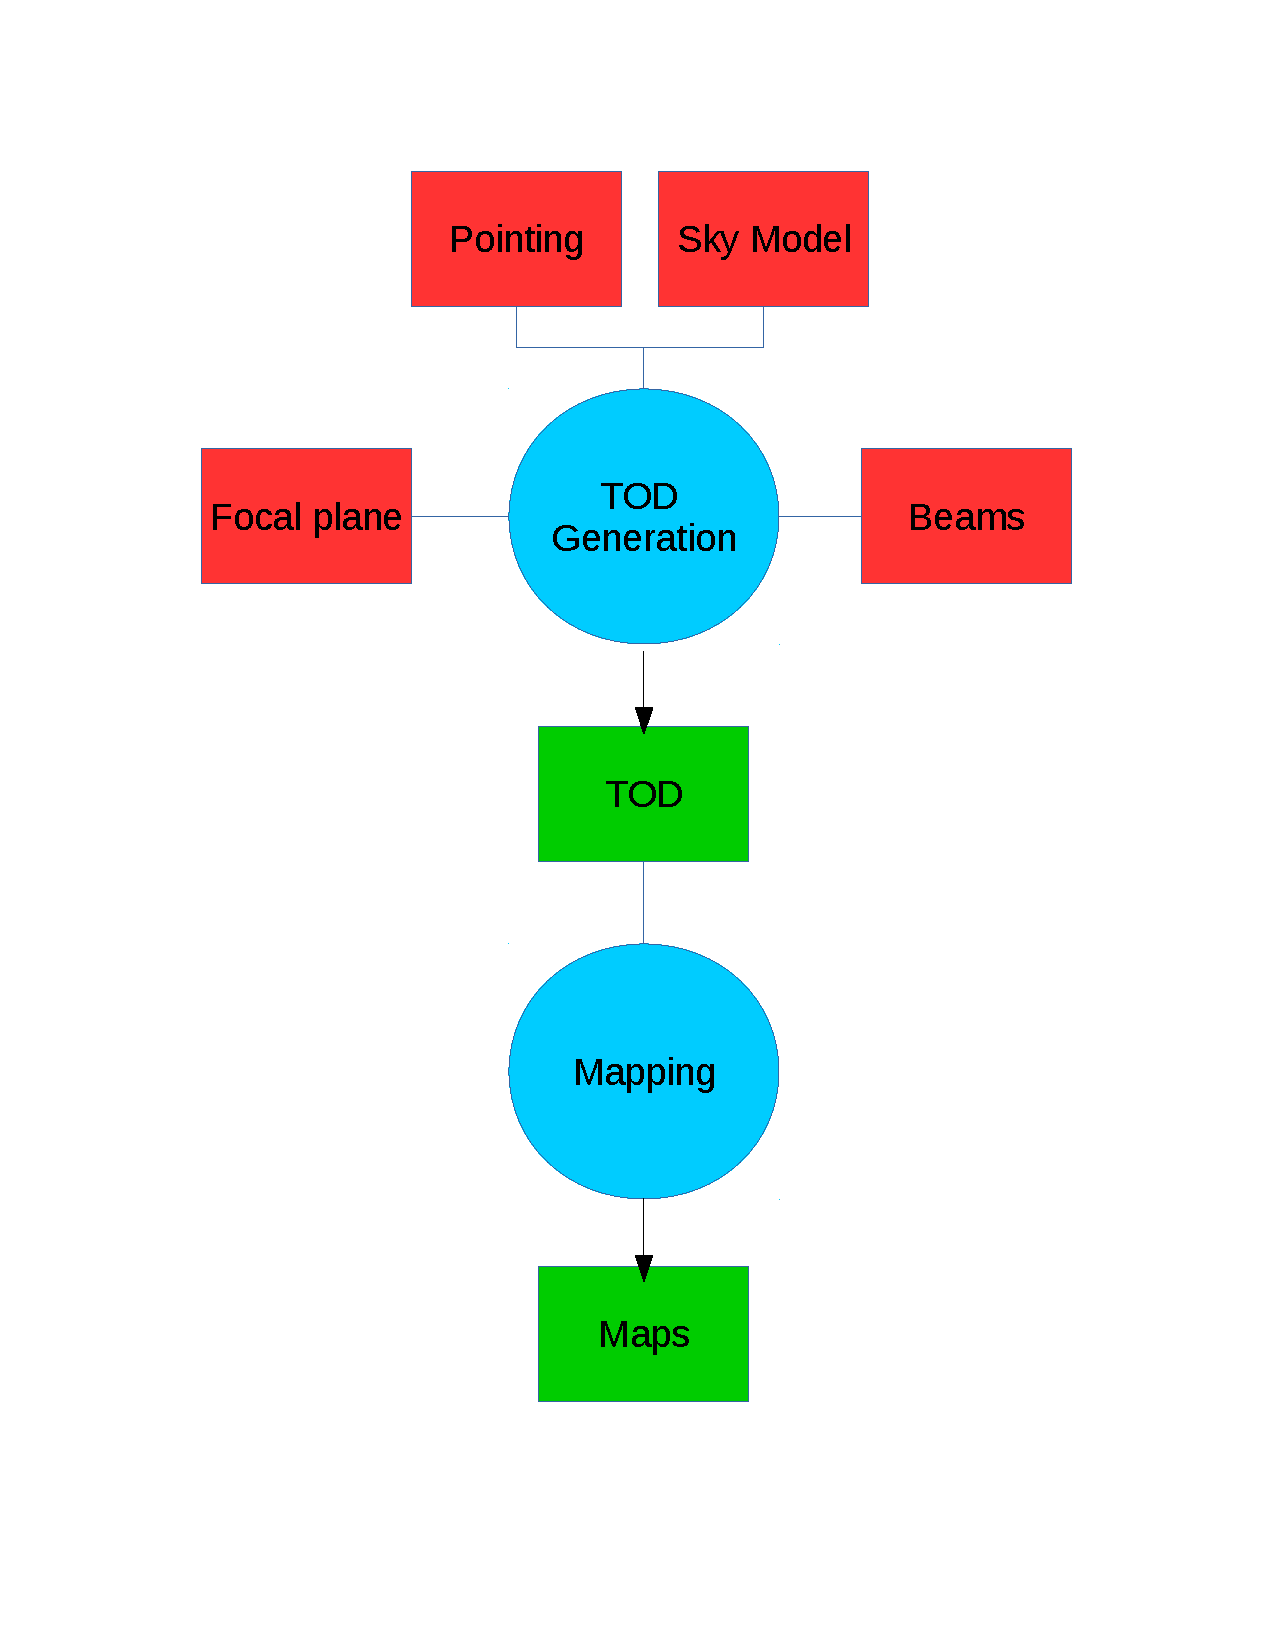
\includegraphics[width=0.6\linewidth]{figures/pisco-flow-diagram}
	\caption{Basic flow of a typical PISCO simulation pipeline. Red polygons show the required user input. PISCO uses this input and produces TOD (green polygon). This TOD stream is calculated using equation \ref{eq::discrete_beam_conv_tensor} for all pointing directions. TOD can then by sent into a mapper and, finally, to a power spectra estimator tool. PISCO does not compute pointing nor produces maps from TOD by itself; these tasks are left to external programs.}
	\label{fig::pisco_flow}
\end{figure}

\subsection{Implementation using CUDA}

\begin{figure}
	\begin{center}
		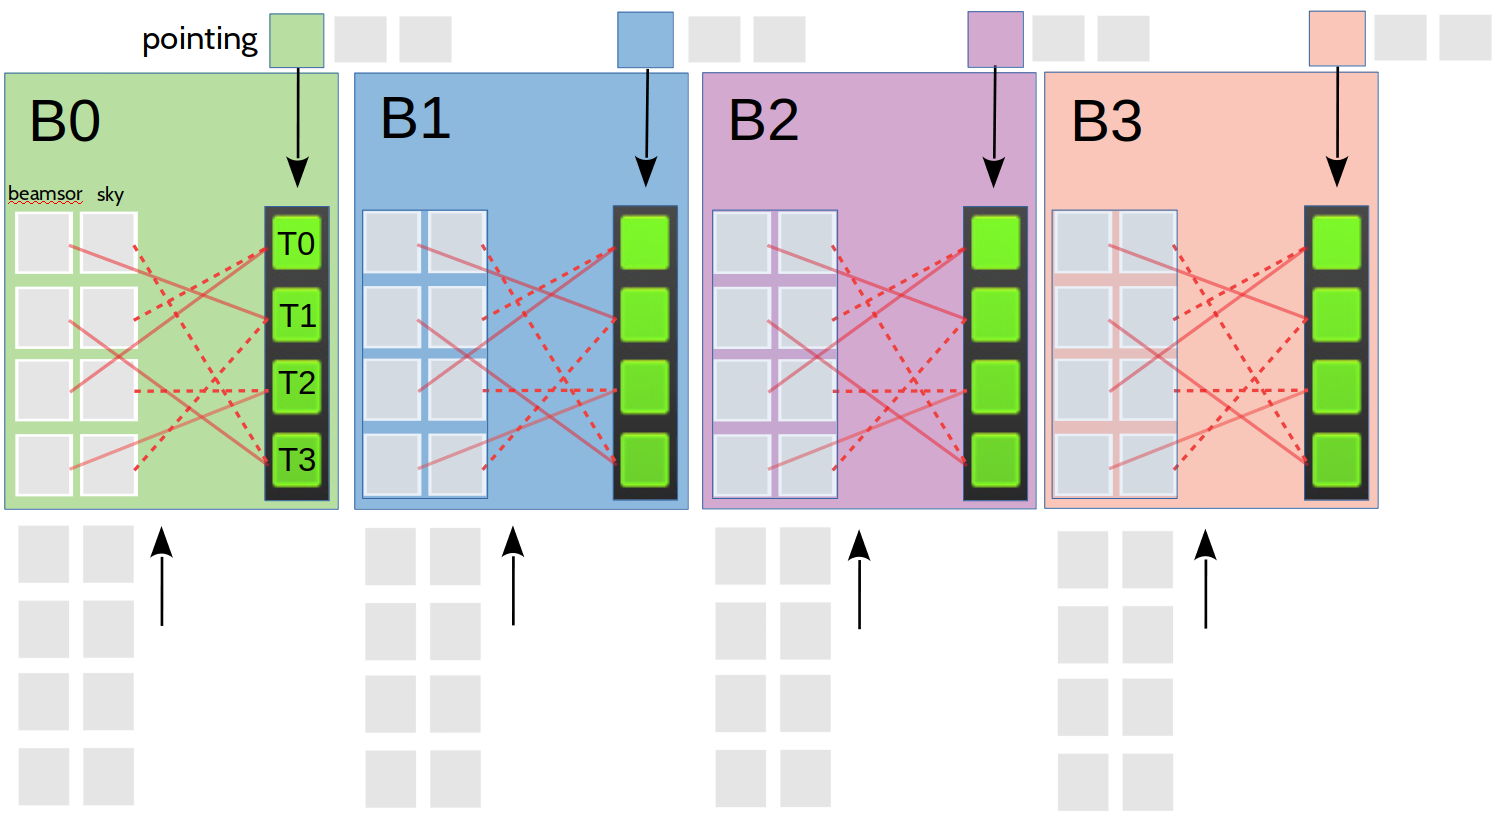
\includegraphics[width=0.8\linewidth]{figures/PISCO-diagram.png}
		\caption{Parallelization scheme. This figure shows the case of PISCO executing in 4 blocks ($B=4$), with four threads per block ($T=4$). Arrays with beamsor and sky elements are at the bottom. Each block has access to four beamsor and sky pixels (gray boxes inside colored boxes) and one pointing entry (colored small boxes) at a time. Green boxes represent the multiplication process of a single beamsor pixel with a single sky pixel. This includes rotating the sky pixel to the antenna polarization basis, and computing the re-pixelization of $B$ at the corresponding coordinates. Solid and dotted red lines represent the complex memory access pattern generated by this process. Every thread within a block writes its result to shared memory space. When a thread finishes its computation, it waits until all threads have finished and a reduction on the shared memory space is performed across all blocks. This process is repeated for every pointing. At the end of the procedure, each block has computed the convolution of a beamsor with the sky for a particular pointing, and every shared memory space of the block has the corresponding result. These results are collected into the GPU global memory, which is then transferred back to CPU (host) memory.}
		\label{fig::pisco_diagram}
	\end{center}
\end{figure}

GPUs allow for substantial acceleration of algorithms that perform a large amount of independent operations. TOD generation using equation \ref{eq::discrete_beam_conv_tensor} presents an optimal application case because all operations are independent of each other. In this work, we used the Compute Unified Device Architecture framework from NVIDIA to implement the TOD generation routine. The reader is referred to \cite{sanders2010cuda} for an excellent description of CUDA and associated capabilities.

To better understand how the parallelism in \ref{eq::discrete_beam_conv_tensor} can exploited, consider the process of synthesizing $N_T$ measurements using a CUDA grid of $B$ blocks and $T$ threads. Consider each measurement to have an associated pointing $\bar{q}_t$ with $t=0..N_T$. PISCO performs a double parallelization scheme: the ``slow'' loop ($L1$) scans the pointing stream and associates every block to a pointing $\bar{q}_t$. A second, ``faster'' loop ($L2$), iterates over a list of pixels, which correspond to sky pixels that are ``inside'' the beamsor extension. This list of pixels is constructed in advance and then transferred to the GPU. $L2$ executes $T$ operations in parallel. Great care was taken to ensure no race conditions arise when multiple threads try to read (write) from (to) the same memory address. As every block executes $T$ convolution operations in parallel, and the CUDA grid runs $B$ simultaneous blocks, the parallelism is $B \times T$. Furthermore, if $G$ GPUs are available, the computation can be distributed among them, increases the parallelism to $G \times B \times T$. A graphical description of this process is shown in figure \ref{fig::pisco_diagram}.

\subsection{Performance}

A simulation of a realistic CMB experiment (see \ref{sec::realistic_cmb_experiment} for more details) took approximately 45 minutes using a node equipped with two Intel Xeon E5-2610 processors (10 physical cores and 20 threads per physical processor), $256$ GB of RAM and one NVIDIA GTX 1080. This simulation generated 1 week of TOD, meaning that PISCO executed around 224 times faster than ``real time operation'' of the experiment. Unfortunately, measuring performance of the current implementation in FLOPS is a highly nontrivial task: the TOD generation routine performs both integer and floating point mathematical operations which are challenging to keep track of. In addition, we were not able to successfully quantify the impact of the memory access pattern caused by having to match beamsor pixels with sky pixels during the convolution step. Nevertheless, and in an effort to provide a comparison basis with other implementations, we claim that this simulation achieved $322560$ convolutions per second. It is quite possible for programs like \texttt{beamconv} (see \cite{2018arXiv180905034D}) to achieve much higher performance than PISCO for this particular test. It is worth noting, however, that PISCO has a small cost associated to increasing the complexity of the beam, i.e., by adding ghosting, high frequency features (in angular space) and time-dependent beam parameters, or transient events on the sky model, like varying temperature of the ground surrounding the receiver. This makes PISCO a good complement to other software tools that perform similar tasks because, while the computational cost might be larger for ``simpler'' cases (highly symmetrical beams and no time-dependent effects), the extra cost of adding another layer of complexity is comparatively low. We also note that, to date, we are not aware of any other software tool that uses the beam tensor formalism explicitly\footnote{In \cite{2007MNRAS.376.1767O}, the authors claim to have performed a ``direct convolution of simulated Stokes maps with the Mueller beams''. Unfortunately, efforts in contacting the authors in order to obtain the source code used for this test were unsuccessful.}

\subsection{Future improvements}

The current implementation must calculate the list of sky pixels involved in each convolution, for all pointing directions, before the CUDA routine is launched. Having this list of pixels in memory decreases the available parallelism, as fewer pointing directions can be used at a given time. While the wall-time associated with this operation is modest, the result must be kept in memory and transferred to the GPU, so that the associated buffer quickly becomes too large to be held in the VRAM. Currently, PISCO handles this situation by performing the generation of TOD in blocks to avoid memory overflow. In the test machine, computing and transferring the lists of pixels can take up to $13\%$ of the \textsl{overall} simulation wall-time. A solution to this problem has already been devised and will be implemented in future releases. Another drawback of the current implementation is the use of global memory to hold the beam tensor elements. Future releases will exploit data locality by making use of the CUDA texture memory pipeline (see \cite{sanders2010cuda}, Chapter 6). Finally, while the current implementation of PISCO was designed to execute in multiple GPU nodes, significant coding effort is required to provide the user with an easy to use interface. Experiments were performed emulating a multi-node system by making PISCO use all 3 GPUs of the machine. These tests showed an almost linear increase in performance, but more work is required in order to find the knee of the curve between performance and available GPUs.

%\begin{table}[tbp]
%	\centering
%	\begin{tabular}{|c|c|c|}
%		\hline
%		Routine description & Time (in seconds) & $\%$ of total time \\
%		\hline
%		convolution & 7967 & 52$\%$  \\
%		query pixel cap & 2171 & 14$\%$ \\
%		transfer pixel cap & 3978 & 27$\%$ \\
%		others & 985 & 7$\%$ \\ 
%		\hline
%	\end{tabular}
%	\caption{Table summarizing the times taken by different routines of PISCO. The simulation executed at more than 19 million convolutions per second.}\label{tbl1}
%\end{table}

% Sub-optimal performance might arise in the case of a slow storage device if a very large amount of pointing data is read from disc. Because of the way PISCO scales in multi-node systems, this situation should be greatly suppressed by using a parallel file-system, so as to exploit data locality and avoid expensive IO operations. We tested a worst case scenario where multiple GPUs read the pointing stream from a single Network Attached Storage (NAS) over a 1 Gigabit Ethernet connection. The pointing stream had more than 870 million individual directions and it was saved to disc as \texttt{NPZ} files. The data was read from the NAS using \texttt{numpy.load}. We found that the IO penalty was less than $5\%$ of the simulation wall-time. We note that this simulation did not write any TOD to disc.

%
\section{Code validation}
\label{sec::validation}

To validate the correctness of PISCO, we performed two sets of tests: a mock observation of a (polarized) point source and a simulation of an ideal CMB observation. All simulations were performed in a machine equipped with three NVIDIA GTX 1080 cards, two Intel Xeon E5-2610 processors (20 physical cores, 40 threads) and $256$ GB of RAM. 

Results from these tests were compared against the \texttt{healpy.smoothing} routine, a Python wrapper around HEALPix routines (see \cite{2005ApJ...622..759G}), which calculates the convolution of a polarized sky with a circularly symmetric Gaussian beam in $a_{\ell m}$ space. For the purposes of this section, we will consider the output of \texttt{smoothing} to be exact. 

\subsection{Point source observations}

The simulated observation of a polarized point source was accomplished by the following steps

\begin{itemize}
	\item Build a beamsor without cross-polarization Each $M_{ii}$ component is a circular Gaussian beam with FWHM of $1.5^\circ$.
	\item Build a $I,Q$ and $U$ skies with a single non-zero pixel at coordinates $(\theta_k,\phi_k)$ The Stokes parameters $S^{i} = (1,Q,U,0)$ of the pixel are set such that $Q^2 + U^2 = 1$ in the polarized cases.
	\item Set up a raster scan around $(\theta_k,\phi_k)$ for a detector with $\zeta=0$. Note that, in order to have full polarization coverage, the raster scan is repeated 3 times with angles $\psi_0 = 0^{\circ},45^{\circ},90^{\circ}$.
	\item Make maps of TOD generated by PISCO.
	\item Compare the result of applying \texttt{smoothing} to the single pixel map using the same beam model.
\end{itemize}

\subsubsection{Results}

Results from this validation test are shown in figure \ref{fig::stokesqsource256beam1024dec45}. The results show that the flux is preserved to better than $0.1\%$. Using a lower \texttt{NSIDE} for the beamsor degrades this considerably. We checked for systematic effects driven by the finite machine precision of the computations, and found that leakage from temperature to polarization is least $10$ orders of magnitude below the maximum amplitude of the Stokes I convolved map. PISCO is also able to correctly account for intra-beam variations of the position angle $\psi$.

\begin{figure}
	\centering
	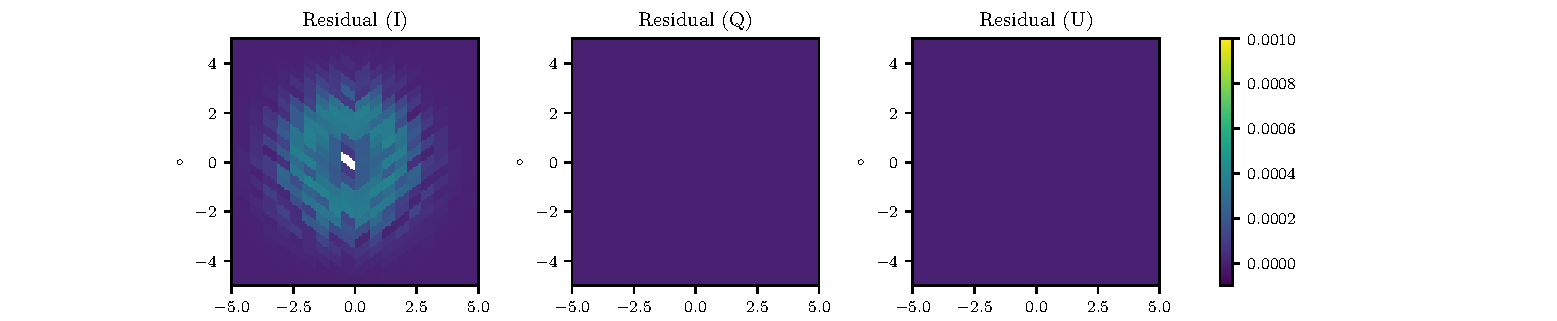
\includegraphics[width=1.0\linewidth]{figures/stokes_I_source_256_beam_1024_dec_45.pdf}
	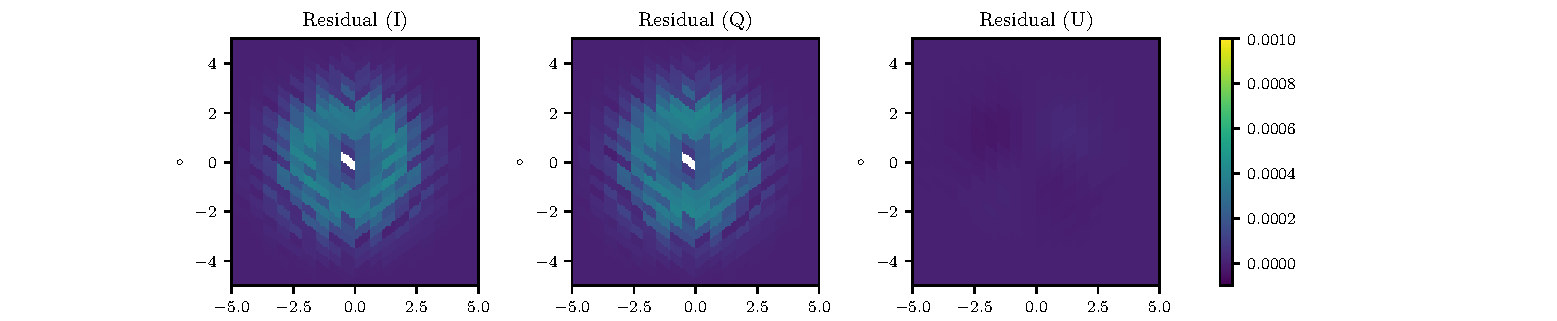
\includegraphics[width=1.0\linewidth]{figures/stokes_Q_source_256_beam_1024_dec_45.pdf}
	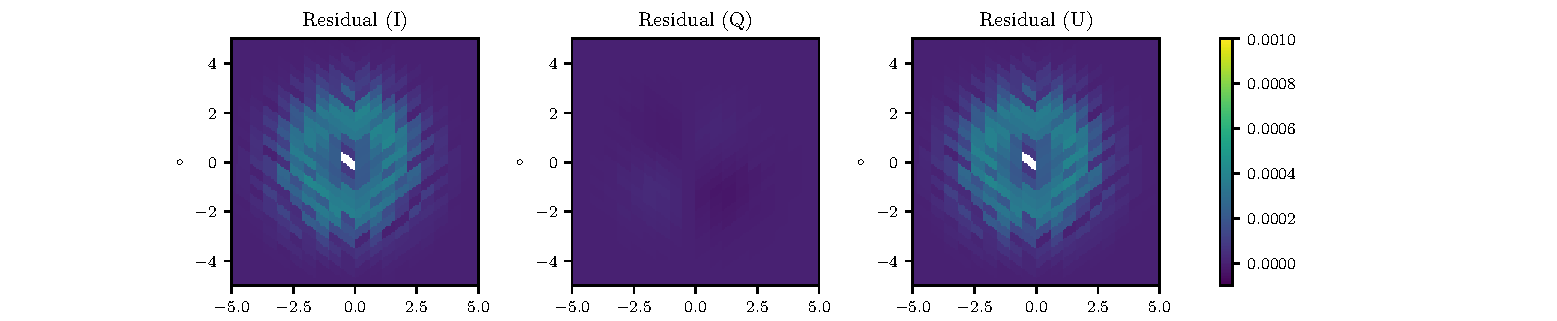
\includegraphics[width=1.0\linewidth]{figures/stokes_U_source_256_beam_1024_dec_45.pdf}
	\caption{Figure showing the results from subtracting a map of a point source convolved with a Gaussian beam using \texttt{smoothing}, and the map generated by PISCO. The input map used HEALPix pixelization with $\mathrm{\texttt{NSIDE}} = 256$. The Beamsor used $\mathrm{\texttt{NSIDE}} = 1024$. The Gaussian profile used for the beamsor had a FWHM of $1.5^\circ$. All point sources were located at $45^\circ$ declination. The color scale is normalized to $1$. From top to bottom: residuals for the case of a point source with Stokes vector $S = (1,0,0,0)$, $S=(1,1,0,0)$ and $S=(1,0,1,0)$, respectively.}
	\label{fig::stokesqsource256beam1024dec45}
\end{figure}

\subsection{Ideal CMB experiment}
\label{sec::ideal_full_sky}

\subsubsection{Description}

As in the point source case, the simulation of an ideal CMB experiment was accomplished by the following:

\begin{itemize}
	\item Build a beamsor without cross-polarization Each $M_{ii}$ component is a circular Gaussian beam with FWHM of $1.5^\circ$.
	\item Build mock CMB whole sky maps with a tensor-to-scalar ratio $r=0.0$.
	\item Set up a scanning strategy to visit each pixel center at 3 different position angles $\psi_0 = 0^{\circ},45^{\circ},90^{\circ}$. 
	\item Make maps of TOD generated by PISCO. 
	\item Compare the maps with a harmonic space convolution of the CMB map with a Gaussian beam.
\end{itemize}

\subsubsection{Sky model}

The input sky maps were generated using a combination of CAMB (see \cite{Lewis:2002ah}) to generate $C_\ell$ and \texttt{synfast} The cosmological parameters correspond to the ones reported by the Planck satellite (see \cite{2016A&A...594A..13P}). This procedure returns 3 CMB anisotropy maps, one for each Stokes parameter\footnote{It is usually assumed the CMB has no circular polarization, so $V$ map was set to zero.} CAMB was configured to return a CMB with no primordial B-modes ($r=0$) and no lensing, as this last effect is expected to produce leakage from E-modes to B-modes. The resulting B-mode power spectrum is effectively zero at all angular scales. No foreground or other sources were added on top of the simulated CMB. All maps use the \texttt{HEALPix} pixelization and were generated at a resolution of \texttt{NSIDE}$=128$. This restricts the analysis in harmonic space to $\ell < 384$.

\subsubsection{Scanning strategy}

The scanning strategy was designed so that every pixel on the sky gets visited exactly three times, each one at a different beam orientation angle. In addition, every pixel is observed at its center, which is an important requirement that ensures the intra-pixel coverage does not affect the estimation of the power spectra at high $\ell$. Since only three hits per pixel at different values of $\psi$ are required to recover the polarization field of the CMB, the scanning was generated for a single detector with a polarization sensitive angle $\zeta=0$.

\subsubsection{Power spectra}

Power spectra were calculated using \texttt{anafast}. No further post-processing of the power spectra were needed given that this simulated observation covers the whole sky, and hence no masking effects arise. The power spectra corresponding to maps that were generated using PISCO TOD were corrected by the equivalent beam transfer function of a circular Gaussian beam of FWHM$=1.5^\circ$. 

\begin{figure}
	\centering
	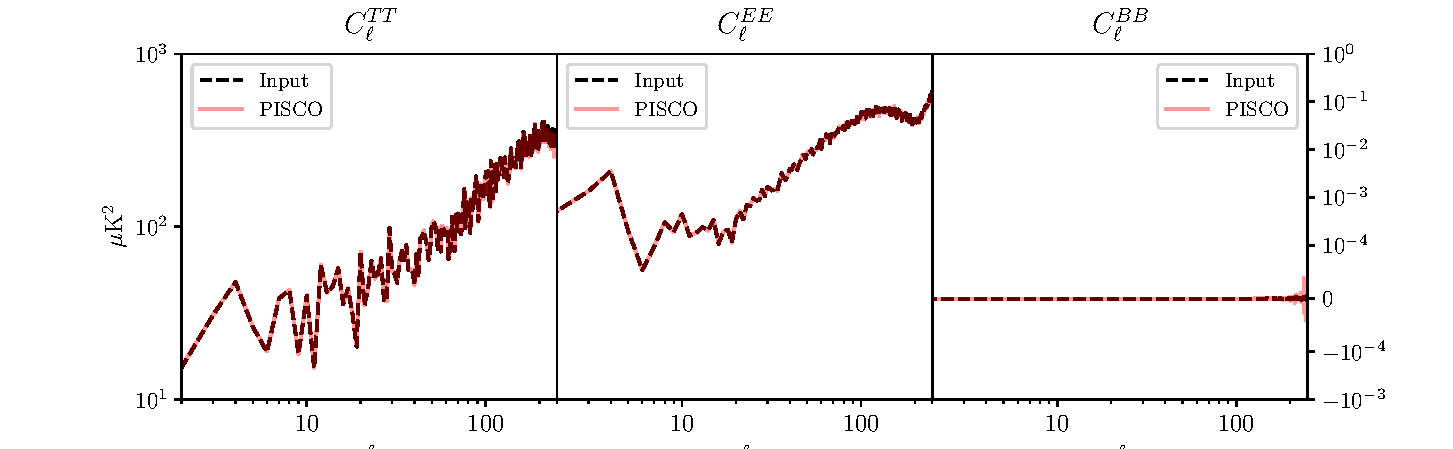
\includegraphics[width=1\linewidth]{figures/cmb_r0d00_CLASS_wholeskytest.pdf}
	\caption{Plots showing maps of PISCO generated TOD and the results from \texttt{smoothing} for whole sky CMB test. Top plot corresponds to power spectra of the input map (blue circles) and the output of PISCO (orange curve) Bottom plot corresponds to the residuals between the input power spectra the one computed from maps generated using PISCO.}
	\label{fig::pisco4wholesky}
\end{figure}

%
\section{Realistic CMB experiment}
\label{sec::realistic_cmb_experiment}

The tests performed above are highly idealized cases. In this section, we show results for a simple, but more realistic application where pointing mismatch, uneven intra-pixel coverage and beam mismatch are present. It has been shown (PF I need citations here) that these mismatches can cause leakage from temperature to polarization. Conversely, uneven intra-pixel coverage can cause divergence in the polarization power spectra at angular frequencies comparable to the pixel size of the input sky map (PF cite Hivon et al). It becomes crucial to check whether PISCO reproduces the effects of these systematic effects correctly in order to validate its performance.
 
\subsection{Description of the simulation}

In this section, we present the procedure and results of a PISCO simulation applied to a more realistic CMB experiment. Since designing a such an experiment from scratch is a challenging task, we turned to simulating an ongoing mission, the Cosmology Large Angular Scale Surveyor, CLASS\cite{2016SPIE.9914E..1KH}. CLASS aims at characterizing the CMB anisotropy field at large angular scales, particularly the power spectra of B-modes and E-modes, looking for evidence of inflation. While the experiment is composed of 4 telescopes, the simulation focuses on the one observing at the lowest frequency (38 GHz), the Q-band receiver. This decision was taken for computational reasons: generating TOD using PISCO scales linearly with the number of detectors and with the length of the pointing stream. Given that CLASS aims at measuring the sky signal over the whole celestial sphere, simulating a receiver with less extended beams requires sampling a higher resolution map than in the case of a wide beam. Consequently, the pointing stream must include more samples in order to not have missing pixels. Similarly, higher frequency receivers have on the order of 500 detectors, while the Q-band receiver only has 72. The combination of fewer detectors and larger beams makes CLASS and its Q-band receiver a good application case to check if PISCO is able to simulate a CMB experiment, using a high-end workstation instead of an HPC facility.

\subsubsection{Sky model}

To generate the maps for this simulation, we followed a similar procedure to the one described in section \ref{sec::ideal_full_sky}. The main difference is the addition of an unpolarized CMB, which was used to check for T to P leakage caused by effects that were not present in section \ref{sec::ideal_full_sky}. All maps use the \texttt{HEALPix} pixelization with an \texttt{NSIDE} parameter of $128$. 

\subsubsection{Pointing}

The scanning strategy of CLASS consists of constant elevation scans (CES). Elevation is kept at $45^{\circ}$ while the telescope rotates $720^\circ$ in azimuth at $1$ degree per second. This process is repeated for around 18 hours per day. The boresight is rotated from $-45^{\circ}$ to $+45^{\circ}$ by $15^{\circ}$ per day on a weekly schedule. This scanning strategy, in combination with the large CLASS field of view results in the telescope covering more than 70 percent of the sky every 24 hours. In addition, because of the boresight rotation, only seven days are needed to provide excellent position angle coverage. Boresight rotation is also key to allowing modulation of both $Q$ and $U$ signals (see \cite{2016SPIE.9914E..1KH}) While CLASS records data $200$ times per second, the pointing streams were generated at $20$ Hz. This down-sampling factor was selected so as not to produce pixel misses, with the median number of hits per pixel being on the order of thousands (PF check this with the plots from mapstats). Down-sampling allows for a ten-fold decrease in computation time.

Taking into account the above considerations, the boresight pointing was generated by closely emulating the scanning strategy in horizontal coordinates (constant elevation scans). Next, the equatorial coordinates for every detector on the focal plane were calculated using this stream and the beam center offsets of the detector. We note that this procedure does not take into account telescope down-time caused by daily maintenance or other systematic effects, like variations in the pointing model. The scanning strategy that was used for this simulation corresponds to seven continuous streams of 24 hours, one for each boresight angle, sampled at $20$ Hz. The pointing stream has more than 870 million individual pointing directions. 

\subsubsection{Beamsor model}

Following the work of \cite{2012SPIE.8452E..20E} and valuable input from the CLASS collaboration, beamsor models for all 72 detectors of the Q-band receiver were built. The two dimensional profile of the diagonal beamsor elements correspond to purely elliptical Gaussian profiles, while the off-diagonal terms were set to zero. The simplicity of the beams allows for further speed-up in the computation by restricting the convolution to a $5^\circ$ disc around the beam center. This value was chosen as, for a unit normalized Gaussian beam, a pixel that is $5^\circ$ away from the centroid of the $1.5^{\circ}$ FWHM beam of the CLASS Q band receiver has a value of $\approx 10^{-14}$, roughly the limit of double precision arithmetic. All beamsors were pixelated using $\rm{NSIDE}=512$. The finite resolution of the beamsor produces an error in the amplitude of simulated TOD that is less than $0.01\%$ compared to analytical estimations, which is consistent with the results described in section \ref{sec::validation}.

%\begin{figure}
%	\centering
%	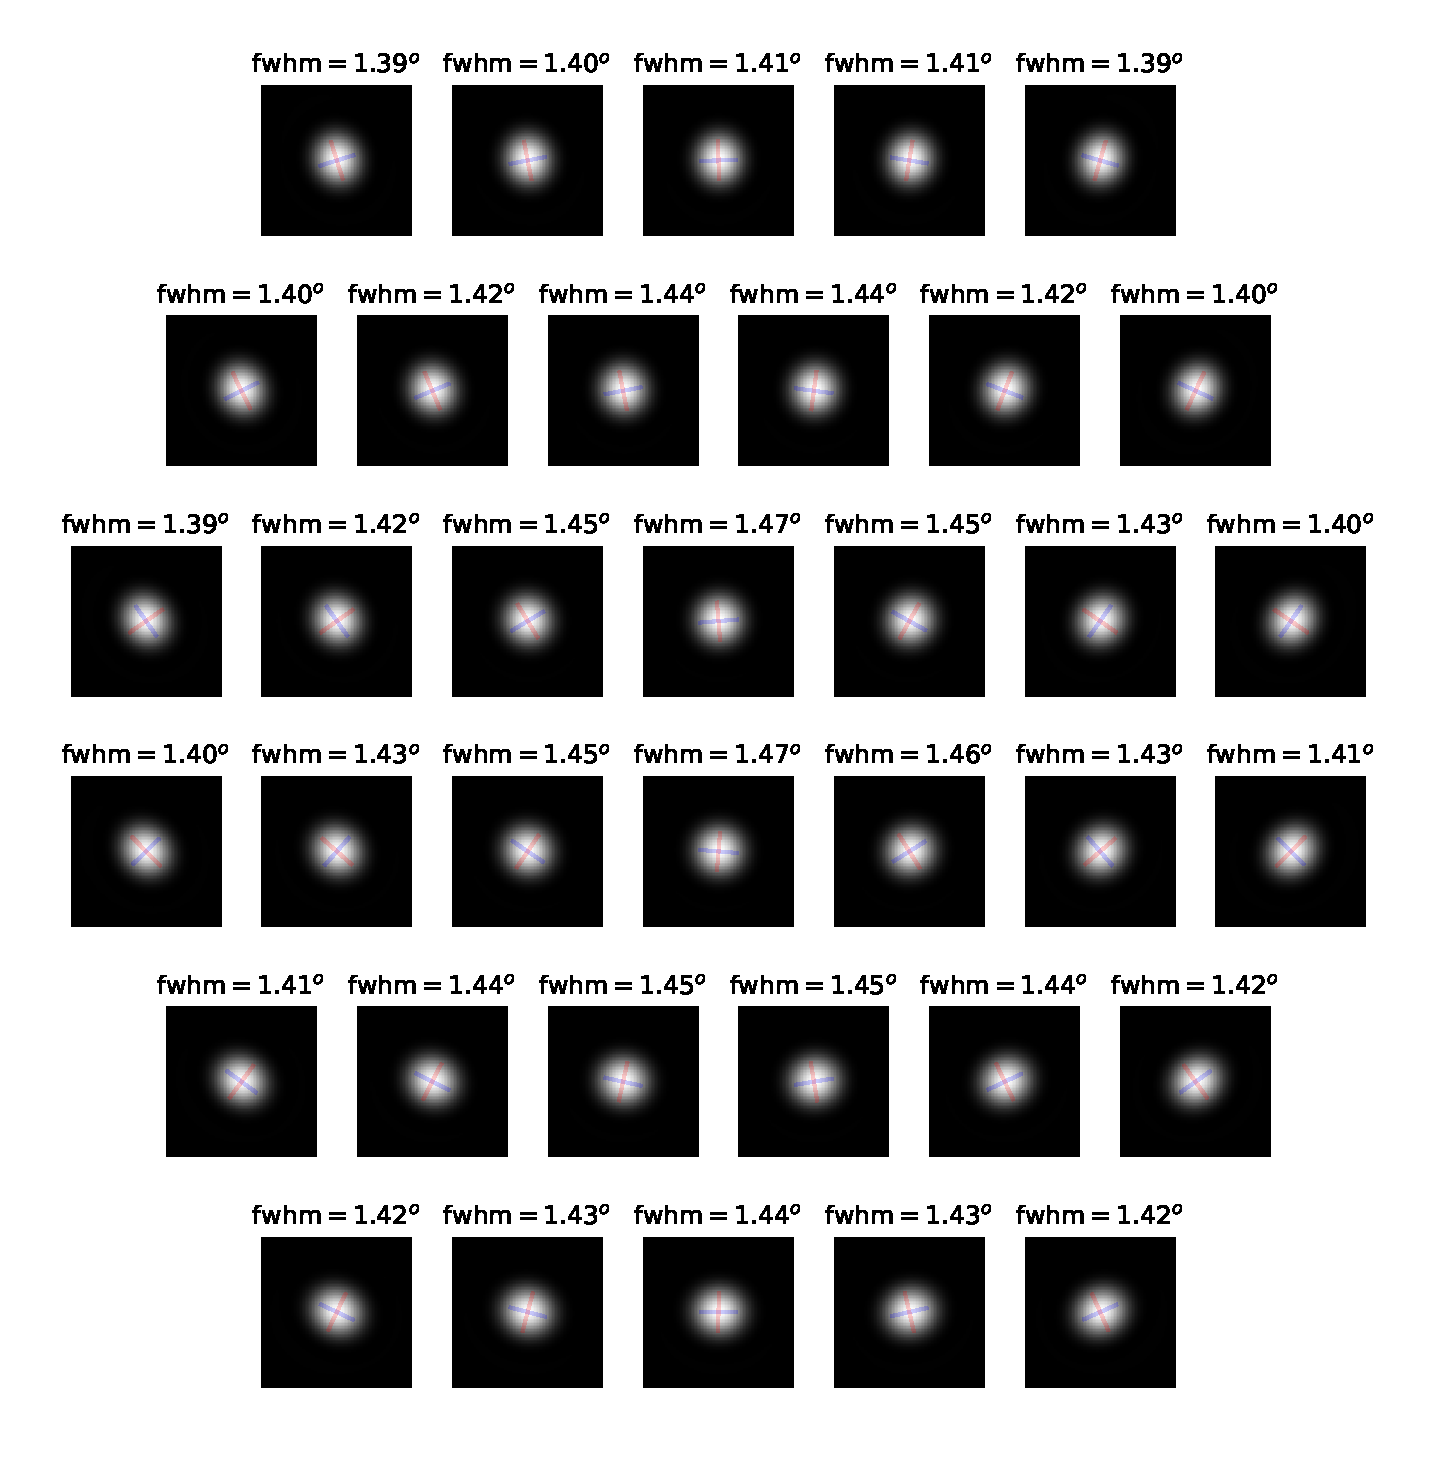
\includegraphics[width=0.8 \linewidth]{figures/qband_beams_main_beam_fwhm_x}
%	\caption{Elliptical Gaussian profiles used as beamsor models for the CLASS Q-band telescope. Relative positions of plots are representative of the positions of feedhorns on the sky. In image coordinates, Zenith is up while East is to the left. All beam profiles are unit normalized, the color scale being linear. Each subplot is a plane projection on the sky of $5^\circ \times 5^\circ$. The title of each subplot is the Full Width at Half Maximum of the profile along its semi-major axis. Non negligible amounts of eccentricity can be seen in the beam profiles, and a visible correlation between beam location on the sky, beam eccentricity and orientation of the major (minor) axis is present. Maximum eccentricity reaches $0.45$ for edge beams.}
%	\label{fig::qbandbeamsmainbeamfwhmx}
%\end{figure}

\subsubsection{Power spectra and beam transfer function}

Given that CLASS only covers $\approx 75\%$ of the sky, computing the power spectra of simulated maps requires the use of a tool than can handle a sky mask. For this reason, we changed the estimator from \texttt{anafast} to \texttt{PolSpice} (PF cite polspice). In addition, the CLASS collaboration provided a realistic sky mask that includes the galactic plane in addition to the natural incomplete coverage. The effect of the beam on the CMB power spectra can be thought as a low-pass filter in harmonic space (cite Page et al) We estimated the equivalent beam transfer function of an arbitrary number of elliptical beams by averaging the radial profiles obtained by by an analytical integration over $\phi$ of all of the beams in ``real'' space and calculating the harmonic transform of the average profile (PF: check this with Mike. I am sure I am missing something! Shall we put this in the appendix as well?)

\subsection{Results and discussion}

\subsubsection{Pointing mismatch}

CMB experiments that rely on detector pairs are subject to leakage caused by pointing mismatch (PF citation needed). Leakage arises at the map-making stage and is caused by an incomplete cancellation of the Stokes $I$ term when solving for the individual pixel-covariance matrices. This residual term from the Stokes $I$ is interpreted by the map-making algorithm as a polarized signal, hence causing the leakage showed in figure \ref{fig::pisco4class_pointingmismatch}. We note that leakage is not present below $\ell \approx 100$, but becomes dominant at increasing angular frequencies. We believe this is caused by the effect of pointing mismatch to be restricted to angular scales comparable to the FWHM of the beam. 

\begin{figure}
	\centering
	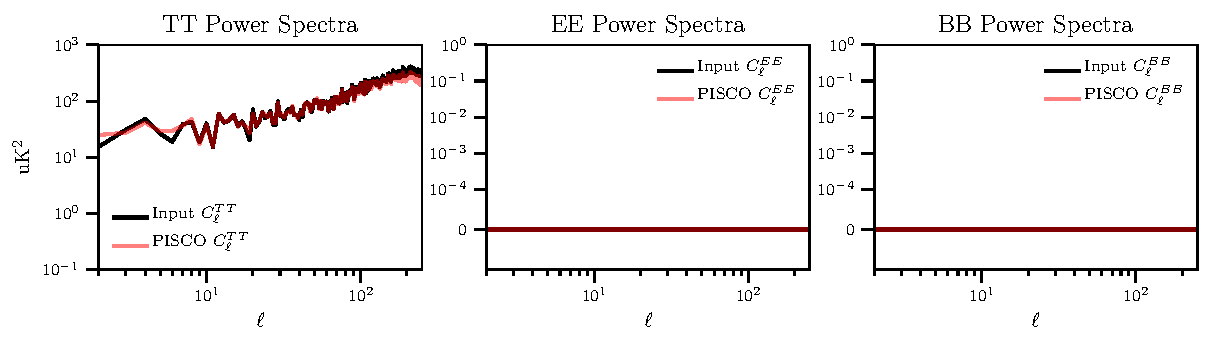
\includegraphics[width=1\textwidth]{figures/unpolCMB_r0d00_CLASS_matchedPointing_matchedBeams_ellipticalBeams.pdf}
	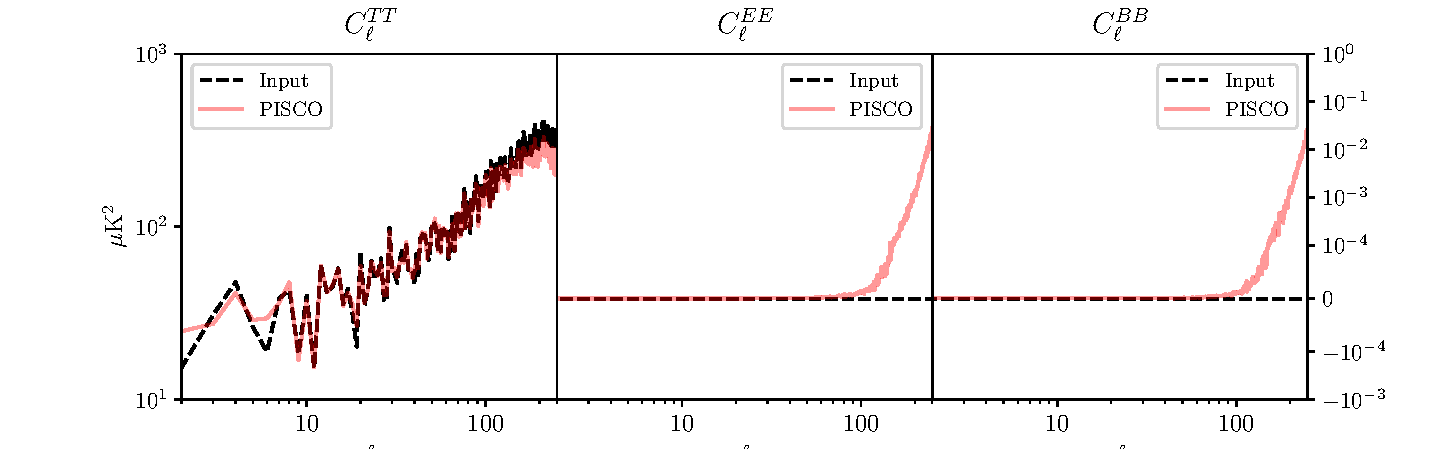
\includegraphics[width=1\textwidth]{figures/unpolCMB_r0d00_CLASS_mismatchedPointing_matchedBeams_ellipticalBeams.pdf}
	\caption{Resulting power spectra for a realistic simulation using mismatched pointing (upper figure), and matched pointing (bottom figure). The input CMB was unpolarized. The amplitude of the mismatch was kindly provided by the CLASS collaboration team. Significant leakage from $TT$ to $EE$ and $BB$ power spectra is present for the mismatched pointing case. The spurious signal reaches in the order of $100$ nK at $\ell = 250$ for both $EE$ and $BB$.}
	\label{fig::pisco4class_pointingmismatch}
\end{figure}

\subsubsection{Uneven intra-pixel coverage}

Simulating a CMB experiment using a more realistic scanning strategy can produce another systematic effect at the power spectra level. This source of noise is related to the intra-pixel coverage of the sky. In section \ref{sec::ideal_full_sky}, all pixels were observed exactly at their centers while, in a real experiments, every sample of the TOD ``hits'' a given pixel at an arbitrary location within it. If, in average, the distribution of hits inside a pixel is symmetric with respect to pixel center coordinates, map-making will average all observations and the power spectra from the resulting map will not be affected. However, if this distribution is asymmetric and gradients between pixels are present (recall that pixel space convolution is affected by neighbor pixels) the resulting power spectra may suffer from P to P leakage. This was discussed in mor detail in (Poutanen et al. 2004) and \cite{2005poutanen}. 

\begin{figure}
	\centering
	%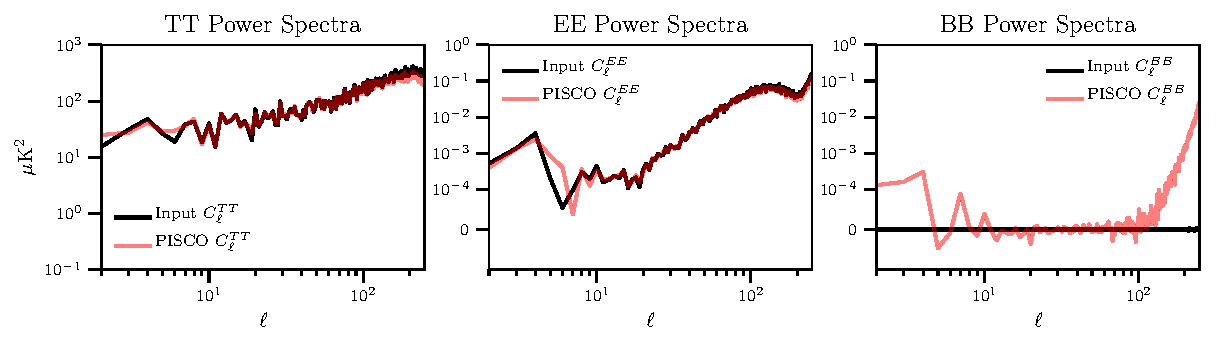
\includegraphics[width=1\textwidth]{figures/cmb_r0d00_CLASS_mismatchedPointing_matchedBeams_ellipticalBeams.pdf}
	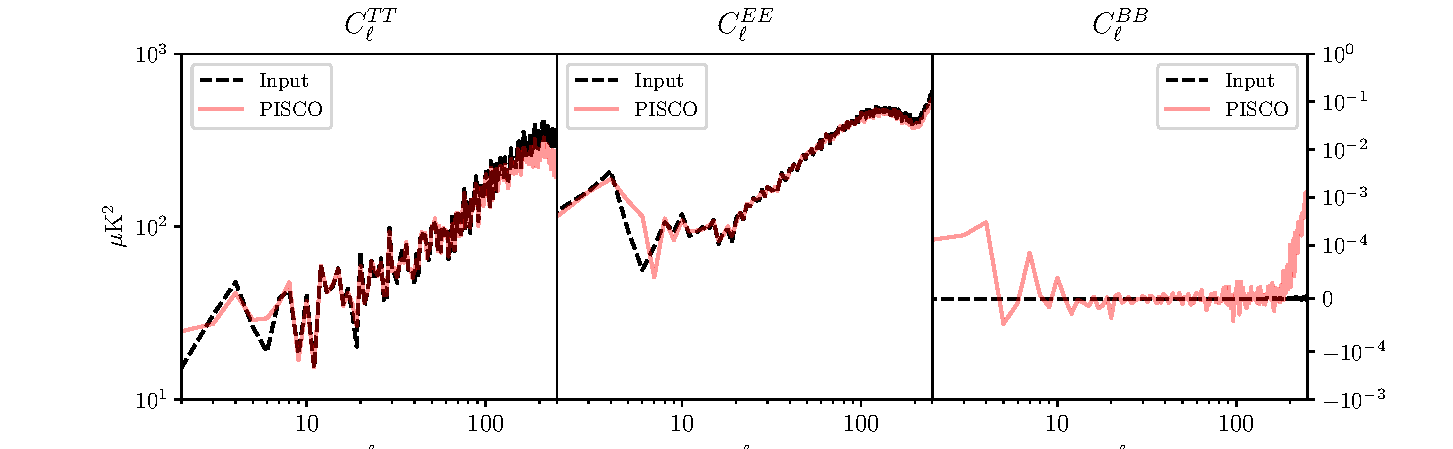
\includegraphics[width=1\textwidth]{figures/cmb_r0d00_CLASS_matchedPointing_matchedBeams_ellipticalBeams.pdf}
	\caption{Resulting power spectra for the case of matched pointing (upper figure), and mismatched pointing (bottom figure), using as input a polarized CMB without B-modes. Both B-mode power spectra show non-negligible amounts of a spurious signal not present in the input power B-mode power spectrum. Both simulation cases (mismatched and matched pointing) also have the effect of uneven intra-pixel coverage. In the case of matched pointing, the spurious B-mode spectrum reaches in the order of $10$ nK at $\ell = 250$.}
	\label{fig::pisco4class_intrapixel}
\end{figure}

Figure \ref{fig::pisco4class_intrapixel} shows the result of running the realistic simulation with matched pointing, and it is clear that a spurious signal is present in the B-mode power spectrum. In the upper plot of Figure \ref{fig::pisco4class_pointingmismatch}, the same simulation was performed but with an unpolarized CMB as input, the resulting polarized power spectra bing consistent with zero. This indicates that the effect of uneven intra-pixel coverage is P to P leakage. We note that this systematic effect is subdominant with respect to the T to P leakage caused by pointing mismatch by roughly a factor of $10$.

\subsubsection{Beam mismatch}

\begin{figure}
	\centering
	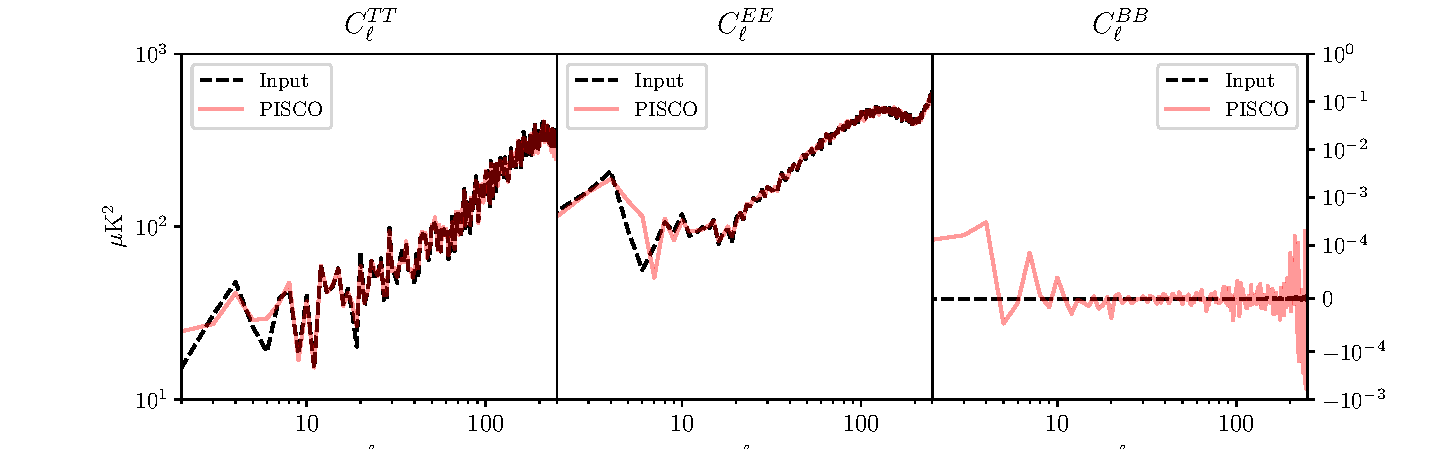
\includegraphics[width=1\textwidth]{figures/cmb_r0d00_CLASS_forcedPointing_matchedBeams_ellipticalBeams.pdf}
	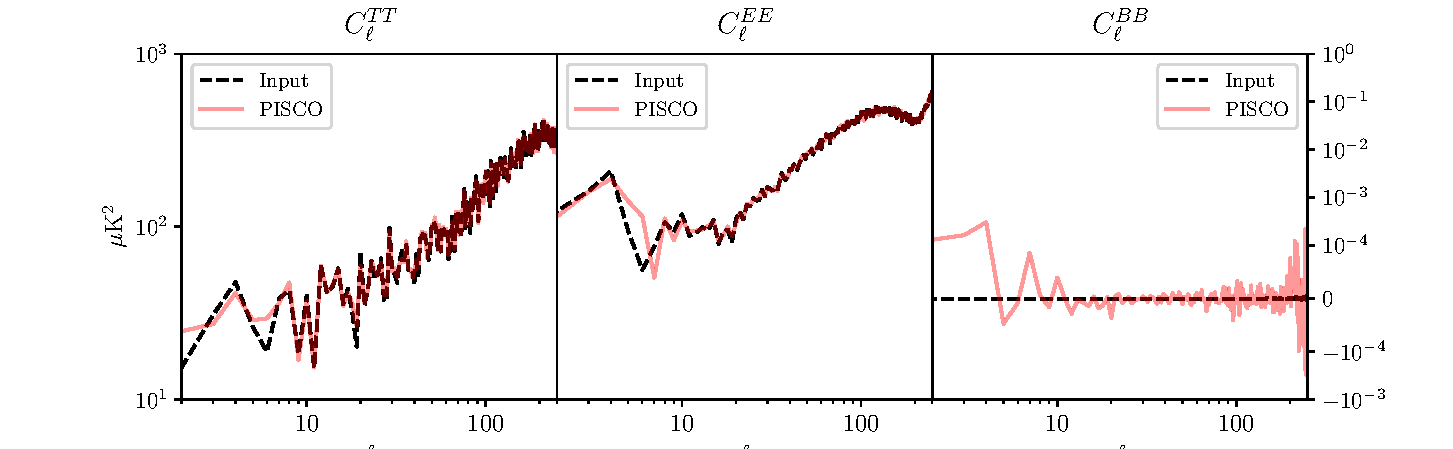
\includegraphics[width=1\textwidth]{figures/cmb_r0d00_CLASS_forcedPointing_mismatchedBeams_ellipticalBeams.pdf}
	\caption{Resulting power spectra of the realistic simulation without the effect of uneven intra-pixel, matched pointing and matched (upper plot) and mismatched (bottom plot) beams. The amplitude of the beam mismatch was kindly provided by the CLASS collaboration team. We see oscillatory behavior in the resulting B-mode power spectrum for both matched and mismatched beam cases. The spurious B-mode signal reaches roughly $100\, \rm{nK}^2$ at $\ell=250$.}
	\label{fig::pisco4class_beammismatch}
\end{figure}

The effect of beam mismatch can be thought as similar to pointing mismatch in that the net effect is to create spurious polarization signal from the temperature field. Beam mismatch can also produce P to P leakage if modulators like Half Wave Plates are present (see \cite{2007MNRAS.376.1767O}). Leakage caused by pointing and beam mismatch are related. Consider the case where the amplitude of the pointing mismatch is comparable to the beam FWHM. In this scenario, paired detectors will effectively be observing different pixels of the sky, making the map-making algorithm interpret the residuals as polarization signals. If the pointing mismatch is small compared to the beam FWHM, this will only happen when one of the paired detectors reaches a pixel border. 

Conversely, beam mismatch changes the way neighboring pixels around a pointing direction are averaged together. For simplicity, consider the case where simple linear transformations are applied to the beams: shear along the $x$ axis and a rotation by an angle $\alpha$ around its center. If the scanning strategy visits all pixels at every possible beam orientation, the effect of the rotation will cancel out the scanning effectively symmetrizes the beam on the sky. The effect of the extension along the $x$-axis will produce leakage from T to P, as every observation with the pair will have slightly different fluxes, and hence a residual, caused by the difference in shape. The mismatch in shape may also cause P to P leakage, particularly near the poles where rapid intra-beam variations will be integrated differently between the pair. We believe this effect to be very small, as the strongest variations of $\psi$ inside the beam happen relatively far away from beam maximum, and are hence weakly weighted by the map-making algorithm.

Figure \ref{fig::pisco4class_beammismatch} shows the resulting power spectra of a simulation with matched pointing, without the effects of uneven intra-pixel coverage and with (without) beam mismatch. Suppressing the effect of intra-pixel coverage systematics was achieved by forcing the pointing of every detector to aim at its closest sky pixel, for an NSIDE resolution of 128. The resulting temperature and E-mode power spectra are in excellent agreement with the input, while the B-mode power spectrum presents some excess signal at large angular scales, as well becoming oscillatory after $\ell=100$. The amplitude of these oscillations reaches $10^{-4} \, \mu\rm{K}^2$, which is an order of magnitude below the effect of intra-pixel coverage. We note, however, that this effect is present in \textsl{both} the matched and mismatched beam cases, and so it is not clear whether this artifact can be associated with beam mismatch. Higher resolution simulations are needed to better constrain this. Unfortunately, this implementation poses a limit on the maximum resolution for beamsors and sky models being used. Future work will address this issue, possibly by making use of multiple GPUs and a more efficient algorithm in terms of memory management.

\section{Conclusion}
\label{sec::conclusions}

In this work, we have presented PISCO, a computer simulation code capable of generating TOD that include the convolution of arbitrary beams and sky models. PISCO exploits the outstanding parallelism that pixel space convolution offers, and implements this using GPU acceleration. PISCO is also designed for efficient execution in HPC environments, particularly, multi-GPU systems. PISCO is unique in its field by using the treatment found in \cite{2007MNRAS.376.1767O} to model the polarization properties of an antenna. In addition, since the core algorithm works in pixel space, we believe that the associated cost of including time-dependent systematic effects and other phenomena is low compared to implementations like the one described in \cite{2018arXiv180905034D}. These systematic effects include, but are not limited to, imperfections in the modulator, beam degradation due to mechanical deformations and transient events of the sky. A paper showing an application of these capabilities to a realistic CMB experiment will be given in future publications.

This work also showed the results from test performed using a pathfinder implementation of the algorithm. With the exception of the test involving beam mismatch, which is inconclusive and needs further investigation, results indicate that PISCO correctly reproduces known systematic effects at the power spectra level. We note that all these test were performed in a high-end workstation, each test taking less than an hour and executing more than 300000 beam convolutions per second.

\bibliographystyle{plain}
\bibliography{bib}

\appendix
%\numberwithin{equation}{section}	
\section{Computation of antenna coordinates from sky coordinates and antenna pointing}

In this appendix we introduce an additional coordinate system, the \textsl{instrument basis} which is a spherical coordinate system with unit base vectors $\hat{x}'$, $\hat{y}'$ and $\hat{z}'$ and spherical coordinates $\theta'$ and $\phi'$. For any given beam center pointing $\bar{q}_0$ in the sky basis, the pointing direction unit vector $\hat{p}_0$ points to the sky at the equator and prime meridian $(\theta'_0,\phi'_0) = (90,0)$ so that the unit vectors $\hat{\theta}'_0$ and $\hat{\phi}'_0$ at that point form the unit base vectors of the antenna basis coordinate system. It is natural for PISCO to adopt Ludwig's 2nd definition of cross polarization \cite{1140406} as this aligns the unit vectors $(\hat{e}_{\co},\hat{e}_{\cx})$ with $(\hat{\theta}',\hat{\phi}')$ for a detector with orientation angle $\zeta = 0$. In particular, this means that, for any beam center pointing $\bar{q}_0 = (90,\phi,0)$ in the sky basis, the co and cross polarization unit vectors are aligned with the Stokes parameters $+U$ and $-U$ respectively across the entire sky.

For a beam center pointing $\bar{q}_0$ and off beam center pointing $\bar{q}$ in the sky basis, we can derive the antenna basis coordinates $(\rho,\sigma)$, the instrument basis coordinates $(\theta',\phi')$ and the angle $\psi$ between $\hat{e}_{\co}$ and $+U$ ($\hat{\theta}$) by using spherical trigonometry (see Figure \ref{fig::figure10}). 

\begin{figure}
	\centering
	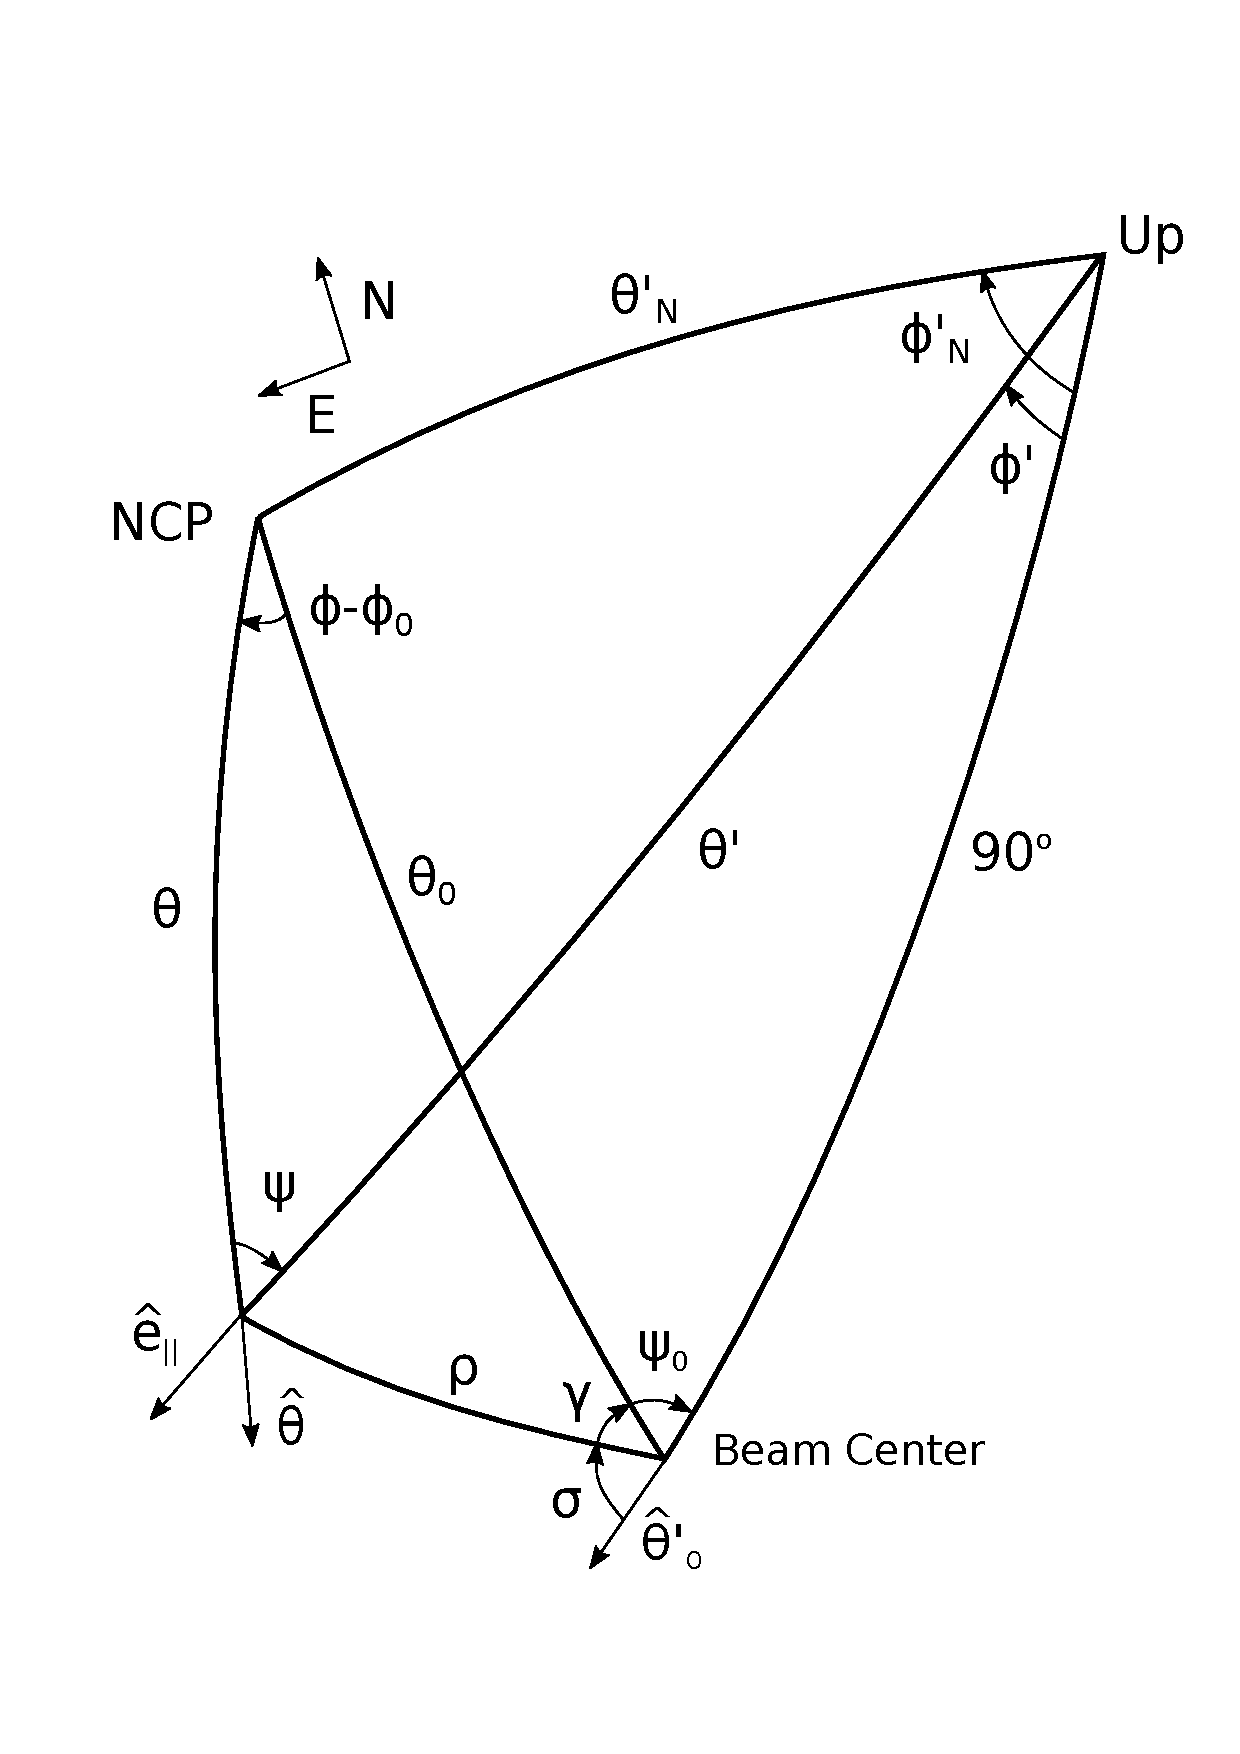
\includegraphics[width=0.8\linewidth]{figures/Figure10.pdf}
	\caption{Sky, instrument and antenna basis coordinates for beam center pointing $\bar{q_0}$ and off beam center pointing $\bar{q}$. Here $\mathrm{\texttt{NCP}}$ is the ICRS North Celestial Pole and $\mathrm{\texttt{Up}}$ is the pole in the upward direction of the instrument basis coordinate system. The instrument basis coordinates of the NCP are $(\theta'_N,\phi'_N)$.}
	\label{fig::figure10}
\end{figure}

Defining $\Delta \phi \equiv \phi - \phi_0$, the antenna basis coordinates $(\rho,\sigma)$ are given by
%
\begin{flalign}
\rho  &= \arccos( \cos(\theta) cos(\theta_0) + \sin(\theta) \sin(\theta_0) \cos(\Delta \phi) ) \nonumber & \\
\sin(\gamma) &= \frac{\sin(\theta) \sin(\Delta \phi)}{\sin(\rho)} \nonumber & \\
\cos(\gamma) &= \frac{\cos(\theta) \sin(\theta_0) - \sin(\theta) \cos(\theta_0) \cos(\Delta \phi)}{\sin(\rho)} & \\ 
\gamma       &=  \arctan \left(\frac{\sin(\theta) \sin(\Delta \phi)}{\cos(\theta) \sin(\theta_0) - \sin(\theta) \cos(\theta_0) \cos(\Delta \phi)} \right) \nonumber & \\
\sigma &= 180^{\circ} - \psi_0 - \gamma \nonumber &
\end{flalign}
%
Then the instrument basis coordinates $(\theta', \phi')$ are
%
\begin{flalign}
\theta' &= \arccos(-\sin(\rho) \cos(\sigma)) \nonumber & \\
\sin(\phi') &= \frac{\sin(\rho) \sin(\sigma)}{\sin(\theta')} \nonumber & \\
\cos(\phi') &= \frac{\cos(\rho)}{\sin(\theta')} & \\
\phi'       &= \arctan \left( \frac{\sin(\rho) \sin(\sigma)}{\cos(\rho)} \right) \nonumber &
\end{flalign}
%
For the instrument basis coordinates $(\theta'_N,\phi'_N)$, we have
%
\begin{flalign}
\theta'_N    &= \arccos(\sin(\theta_0) \cos(\psi_0)) \nonumber & \\
\sin(\phi'_N) &= \frac{\sin(\theta_0)  \sin(\psi_0)}{\sin(\theta'_N)}  & \\
\cos(\phi'_N) &= \frac{\cos(\theta_0)}{\sin(\theta'_N)} \nonumber & \\ 
\phi'_N       &= \arctan\left( \frac{\sin(\theta_0)  \sin(\psi_0)}{\cos(\theta_0)} \right) \nonumber &
\end{flalign}
%
Then, defining $\Delta \phi' \equiv \phi'_N - \phi'$, yields
%
\begin{flalign}
\cos(\psi) &= \frac{\cos(\theta'_N) \sin(\theta') - \sin(\theta'_N) \cos(\theta') \cos(\Delta \phi')}{\cos(\theta)}  \nonumber & \\
\sin(\psi) &= \frac{\sin(\theta'_N) \sin(\Delta \phi')}{\cos(\theta)}  & \\
\psi       &= \arctan\left( \frac{\sin(\theta'_N) \sin(\Delta \phi')}{\cos(\theta'_N) \sin(\theta') - \sin(\theta'_N) \cos(\theta') \cos(\Delta \phi')} \right)  \nonumber &
\end{flalign}

\section{Calculation of elements of $B$}

A beamsor $B$ evaluated at antenna basis coordinates $(\rho,\sigma)$ is a $4 \times 4$ matrix with elements

\begin{equation}
\begin{aligned}
B(\rho,\sigma) = \frac{1}{\tilde{\Omega}}
\begin{bmatrix}
B_{TT} & B_{QT} & B_{UT} & B_{VT}\\
B_{TQ} & B_{QQ} & B_{UQ} & B_{VQ}\\
B_{TU} & B_{QU} & B_{UU} & B_{VU}\\
B_{TV} & B_{QV} & B_{UV} & B_{VV}
\end{bmatrix}
\end{aligned}
\label{eq::beamsor_appendix}
\end{equation}

\noindent
with $\tilde{\Omega}$ being a normalization factor computed as

\begin{equation}
\begin{aligned}
\tilde{\Omega} = \int_{4\pi} B_{TT}(\rho,\sigma) \, \mathrm{d} \Omega
\end{aligned}
\end{equation}

The definition of a beamsor used in this work differs from the one listed in \cite{2007MNRAS.376.1767O} in that element $B_{XY}$ corresponds to element $B_{YX}$. We believe this definition yields a clearer interpretation of beamsor elements. Consider, for instance, the product of $B$ with a Stokes vector representing an unpolarized source. This yields

\begin{equation}
\begin{aligned}
\begin{bmatrix} 
B_{TT} \\ 
B_{TQ} \\ 
B_{TU} \\ 
B_{TV} 
\end{bmatrix}
=
\begin{bmatrix}
B_{TT} & B_{QT} & B_{UT} & B_{VT}\\
B_{TQ} & B_{QQ} & B_{UQ} & B_{VQ}\\
B_{TU} & B_{QU} & B_{UU} & B_{VU}\\
B_{TV} & B_{QV} & B_{UV} & B_{VV}
\end{bmatrix}
\cdot
\begin{bmatrix} 
1 \\ 
0 \\ 
0 \\ 
0 
\end{bmatrix}
\end{aligned}
\label{eq::unpol_beamsor}
\end{equation}

\noindent
where it is more evident that elements $B_{TX}$, with $X=Q,U,V$, correspond to the temperature to polarization leakage beams. 

In most CMB applications, linearly polarized detectors are placed at the focus of the antenna. In general, power that was radiated as pure $+Q$ in the detector basis will reach the sky as both $+Q$ and $-Q$ in the antenna basis. This effect can be modeled by introducing co-polar and cross-polar beams. The co-polar beam, $b_{\co}(\rho,\sigma)$, is the unit-normalized power density distribution that reaches the sky with a polarization state parallel to $\hat{e}_{\co}$. The cross-polar $b_{\cx}(\rho,\sigma)$ does so parallel to $\hat{e}_{\cx}$. 

The work of \cite{2007A&A...470..771J} also provides a way of calculating beamsor elements. Given the coordinate system convention used in this work, it is important to re-specify the way these elements are calculated. We start by considering the antenna to broadcast power originated by a linearly polarized source radiating at the location of the detection device. This will produce a distribution of electric fields in the far field, $\vec{E} = \vec{E}(\rho,\sigma)$, where $\vec{E}(\rho,\sigma)$ will have co-polarized and cross polarized components. Take $x$ to be a source oriented such that most of its radiated power reaches the sky as electric fields aligned with $\hat{\theta}'$ at beam center. Similarly, consider another source, $y$, aligned perpendicularly such that most its transmitted power reaches the sky as electric fields aligned with $\hat{\phi}'$, at beam center. In this situation, elements of a beamsor can be computed via

\begin{equation}
\begin{split}
B_{TT}&=\frac{1}{2}\left(\left|\vec{E}_{x}\right|^{2}+\left|\vec{E}_{y}\right|^{2}\right)\\
B_{QT}&=\frac{1}{2}\left(\left|\vec{E}_{x,\co}\right|^{2}-\left|\vec{E}_{x,\cx}\right|^{2} +  \left|E_{y,\cx}\right|^{2}-\left|E_{y,\co}\right|^{2}\right)\\
B_{UT}&=\frac{1}{2}\left(\vec{E}_{x,\co} E_{x,\cx}^{*} - E_{y,\co} E_{y,\cx}^{*}\right) + \mathrm{c.c.}\\
B_{VT}&=\frac{1}{2}\mathrm{i}\left(\vec{E}_{x,\co}\vec{E}_{x,\cx}^{*} + \vec{E}_{y,\co} \vec{E}_{y,\cx}^{*}\right) + \mathrm{c.c.}\\
B_{TQ}&=\frac{1}{2}\left(\left|\vec{E}_{A}\right|^{2}-\left|\vec{E}_{B}\right|^{2}\right)\\
B_{QQ}&=\frac{1}{2}\left(\left|\vec{E}_{x,\co}\right|^{2}-\left|\vec{E}_{x,\cx}\right|^{2}+\left|\vec{E}_{y,\co}\right|^{2}-\left|\vec{E}_{y,\cx}\right|^{2}\right)\\
B_{UQ}&=\frac{1}{2}\left(\vec{E}_{x,\co} \vec{E}_{x,\cx}^{*} + \vec{E}_{y,\co} \vec{E}_{y,\cx}^{*}\right)+\mathrm{c.c.}\\
B_{VQ}&=\frac{1}{2}\mathrm{i}\left( \vec{E}_{x,\co} E_{x,\cx}^{*} - E_{y,\co} E_{y,\cx}^{*}\right)+\mathrm{c.c.}\\
B_{TU}&=\frac{1}{2}\left( -\vec{E}_{x,\co} \vec{E}_{x,\cx}^{*} + \vec{E}_{y,\cx} \vec{E}_{y,\co}^{*}\right)+\mathrm{c.c.}\\
B_{QU}&=\frac{1}{2}\left(-\vec{E}_{x,\co}\vec{E}_{y,\cx}^{*} - \vec{E}_{x,\cx} \vec{E}_{y,\co}^{*}\right)+\mathrm{c.c.}\\
B_{UU}&=\frac{1}{2}\left(\vec{E}_{x,\co} \vec{E}_{y,\co}^{*} - \vec{E}_{x,\cx} \vec{E}_{y,\cx}^{*}\right)+\mathrm{c.c.}\\
B_{VU}&=\frac{1}{2}\mathrm{i}\left(\vec{E}_{x,\co} \vec{E}_{y,\co}^{*} + \vec{E}_{x,\cx}\vec{E}_{y,\cx}^{*}\right)+\mathrm{c.c.}\\
B_{TV}&=\frac{1}{2}\mathrm{i}\left(\vec{E}_{x,\co} \vec{E}_{y,\cx}^{*} - \vec{E}_{x,\cx}\vec{E}_{y,\co}^{*}\right)+\mathrm{c.c.}\\
B_{QV}&=\frac{1}{2}\mathrm{i}\left(\vec{E}_{\mathrm{x,\co}} \vec{E}_{y,\cx}^{*} + \vec{E}_{x,\cx} \vec{E}_{y,\co}^{*}\right)+\mathrm{c.c.}\\
B_{UV}&=\frac{1}{2}\mathrm{i}\left(-\vec{E}_{x,\co} \vec{E}_{y,\co}^{*} + \vec{E}_{A,\cx} \vec{E}_{y,\cx}^{*}\right)+\mathrm{c.c.}\\
B_{VV}&=\frac{1}{2}\left(\vec{E}_{x,\co} \vec{E}_{y,\co}^{*} + \vec{E}_{x,\cx} \vec{E}_{y,\cx}^{*}\right)+\mathrm{c.c.}
\end{split}
\end{equation}
%
\noindent
where c.c. stands for complex conjugate.

\end{document}
